\documentclass[pldi]{sigplanconf}

% \newcommand{\ignore}[1]{}

%% =============================================================
\def\tool{\textsc{Clotho}\xspace}
%\def\papertitle{\tool: Program Repairing using Exception Types, Constraint
%Automata and Typestate}
\def\papertitle{\tool: Saving Programs from Malformed Strings and Incorrect
String-handling}
\def\pdfauthors{}
\def\paperkeywords{}
%% =============================================================

\usepackage{color}

\newcommand{\subparagraph}{}

% You can tweak clickable link colors here:
\definecolor{linkcol}{rgb}{0,0,1}
\definecolor{citecol}{rgb}{0,0.5,0}
\definecolor{urlcol}{rgb}{0.3,0,0}

% Make pdflatex use letter size --md
\setlength{\pdfpagewidth}{8.5in}
\setlength{\pdfpageheight}{11in}

\let\proof\relax
\let\endproof\relax

\usepackage{cite}
\usepackage{amsthm}
% \usepackage{amsmath}
% \usepackage{amsfonts}
\usepackage{ragged2e}
\usepackage{txfonts}
\usepackage{fancyhdr}
\usepackage{amssymb}
\usepackage{fancyvrb}
\usepackage{graphicx}
\usepackage{times}
\usepackage{pifont}
\usepackage[hyphens]{url}
\usepackage{xspace}
\usepackage{sty/algorithm2e}
%%\usepackage[belowskip=-10pt,aboveskip=5pt,small,labelfont=bf]{caption}
\usepackage[aboveskip=5pt,small,labelfont=bf]{caption}
\DeclareCaptionType{copyrightbox}
\usepackage[bookmarks=true,%
bookmarksnumbered=true,%
colorlinks=true,%
linkcolor=linkcol,%
citecolor=citecol,%
urlcolor=urlcol,%
hypertexnames=true,%
pdfpagelabels,
% draft
]{hyperref}

\hypersetup{%
  colorlinks=false,% hyperlinks will be black
  pdfborderstyle={/S/U/W 1}% border style will be underline of width 1pt
}

\usepackage{sty/multirow}
\usepackage{sty/flushend}
\usepackage{epstopdf}
\usepackage[small,compact]{sty/titlesec}
\usepackage[font=scriptsize]{subfig}
\usepackage{sty/wrapfig}

\usepackage{epstopdf}
\usepackage{fancybox}
\usepackage{listings}
\usepackage{xcolor}
%\usepackage[]{datetime}
%\usepackage{lipsum}

\newcommand{\ignore}[1]{}
% \usepackage{rotating}

%==========================================
%Added definitions
% \usepackage{amsthm}
\theoremstyle{definition}
\newtheorem{definition}{Definition}[section]
%==========================================
%rename listing
\renewcommand\lstlistingname{Code}
%==========================================

%==========================================
%rotate column title
\usepackage{booktabs}
% \usepackage{xparse}
% \NewDocumentCommand{\rot}{O{45} O{1em} m}{\makebox[#2][l]{\rotatebox{#1}{#3}}}
%==========================================

%==========================================
%Automatic row number in table
% \usepackage{array,etoolbox}
% \preto\tabular{\setcounter{magicrownumbers}{0}}
% \newcounter{magicrownumbers}
% \newcommand\rownumber{\stepcounter{magicrownumbers}\arabic{magicrownumbers}}
%==========================================
\SetAlFnt{\small}
\SetAlCapFnt{\small}
\SetAlCapNameFnt{\small}
\SetVlineSkip{0pt}

\setlength\floatsep{5pt}
\setlength\textfloatsep{5pt}
\setlength\intextsep{5pt}

\hypersetup{
pdfauthor = {},
pdftitle = {\papertitle},
pdfkeywords = {\paperkeywords},
pdfcreator = {LaTeX with hyperref package},
pdfproducer = {pdflatex}}

\definecolor{dkgreen}{rgb}{0,0.6,0}
\definecolor{gray}{rgb}{0.5,0.5,0.5}
\definecolor{mauve}{rgb}{0.58,0,0.82}

\lstset{%frame=tb,
  captionpos=b,
  language=Java,
  aboveskip=10pt,
  belowskip=0pt,
  abovecaptionskip=5pt,
  belowcaptionskip=5pt,
  numberblanklines=false,
  showstringspaces=false,
  columns=flexible,
  basicstyle={\scriptsize\ttfamily},
  numbers= left,
  numbersep=5pt,
  numberstyle=\scriptsize,
  %frame=single,
  numberstyle=\tiny\color{gray},
  keywordstyle=\color{blue},
  commentstyle=\color{dkgreen},
  stringstyle=\color{mauve},
  breaklines=true,
  breakatwhitespace=true
  tabsize=2,
  xleftmargin=2em,
  morecomment=[l]{//},
  escapeinside={<@}{@>},
}

\makeatletter
\lst@Key{countblanklines}{true}[t]%
    {\lstKV@SetIf{#1}\lst@ifcountblanklines}

\lst@AddToHook{OnEmptyLine}{%
    \lst@ifnumberblanklines\else%
       \lst@ifcountblanklines\else%
         \advance\c@lstnumber-\@ne\relax%
       \fi%
    \fi}
\makeatother

% Use a smaller font size for URLs:
\makeatletter
\def\url@myurlstyle{%
   \@ifundefined{selectfont}{\def\UrlFont{\small}}{\def\UrlFont{\small}}}
   \makeatother
\urlstyle{myurl}

% This adds ':' to the characters after which not to break URLs, and
% defines a smaller typewriter font. --cpk
% changed small to sf -- md
\def\UrlNoBreaks{\do:\do\(\do\[\do\{\do\<}%
\def\UrlFont{\small\ttfamily}
\def\UrlOrds{\do\*\do\~}%

% For referencing sections, Vern-style
\newcommand\xref[1]{\S~\ref{#1}}

% Black filled circles with white number on it
% See Comprehensive LaTeX Symbol List --cpk
\def\blackI{\ding{182}}
\def\blackII{\ding{183}}
\def\blackIII{\ding{184}}
\def\blackIV{\ding{185}}
\def\blackV{\ding{186}}
\def\blackVI{\ding{187}}

\def\first{({\it i})\xspace }
\def\second{({\it ii})\xspace }
\def\third{({\it iii})\xspace }
\def\fourth{({\it iv})\xspace }
\def\fifth{({\it v})\xspace }

% For notes to authors:
\newcommand{\note}[1]{{\textcolor{red}{[\textit{#1}]}}}

% Fine-tuning for table spacing. --cpk
\def\TblSpT{\rule[-1ex]{0pt}{0pt}}
\def\TblSpB{\rule{0pt}{2.5ex}}

% Squeezing out some space. --cpk
% http://www-h.eng.cam.ac.uk/help/tpl/textprocessing/squeeze.html
%
%\renewcommand\subfigtopskip{0pt}
%\renewcommand\subfigbottomskip{5pt}
%\renewcommand\subfigcapskip{0pt}
%\renewcommand\floatpagefraction{.9}
%\renewcommand\topfraction{.9}
%\renewcommand\bottomfraction{.9}
%\renewcommand\textfraction{.1}
%\setlength{\parskip}{0em}
%\frenchspacing


%%%%%%%%%%%%%%%%%%%%%%%%%%%%%%%%%%%%%%%%%%%%%%%%%
% \hyphenpenalty 10000
% \exhyphenpenalty 10000
\sloppy
%%%%%%%%%%%%%%%%%%%%%%%%%%%%%%%%%%%%%%%%%%%%%%%%%

\newcommand{\comment}[1]{{\color{red}#1}}
\newcommand{\code}[1]{\texttt{\scriptsize{#1}}}
\newcommand{\mycomment}[1]{}
\newcommand{\todo}[1]{\textbf{TODO: #1}}
\newcommand{\mytab}{~~~~}
\newcommand{\sspace}{~}
\newcommand{\etal}{\textit{et al.}}
\newcommand{\eg}{{e.g.,}}
\newcommand{\ie}{{i.e.,}}
\newcommand{\lno}[1]{{\tiny{\textbf{(#1)~~}}}}

\newcommand{\java}{\textsc{Java}}
\newcommand{\soot}{\textsc{Soot}}
\newcommand{\infoflow}{\textsc{InfoFlow}}
\newcommand{\sdn}{{SDN}}
\newcommand{\verifier}{\textsc{Verifier}}
\newcommand{\validator}{\textsc{Flow\_Consistency\_ Validator}}
\newcommand{\outputs}{{\mathbb O}}
\newcommand{\stream}{{\mathbb S}}
\SetEndCharOfAlgoLine{}

%% for IEEEtran
\def\tablename{Table}

\renewcommand{\thetable}{\arabic{table}}

\newcommand*{\refname}{Bibliography}

\def\yes{\ding{51}}
\def\no{\ding{55}}

%------------------------------------------------------------------------------
%                                Space savers.
%------------------------------------------------------------------------------
% This mylist environment indents items, and saves less space than the above.
\newcounter{myctr}
\newenvironment{mylist}{\begin{list}{(\textbf{\arabic{myctr}})}
{\usecounter{myctr}
\setlength{\topsep}{1mm}\setlength{\itemsep}{0.5mm}
\setlength{\parsep}{0.5mm}
\setlength{\itemindent}{0mm}\setlength{\partopsep}{0mm}
\setlength{\labelwidth}{-2mm}
\setlength{\leftmargin}{0mm}}}{\end{list}}

% Space saving List environment for itemizing.
\newenvironment{mybullet}{\begin{list}{$\bullet$}
{\setlength{\topsep}{1mm}\setlength{\itemsep}{0.5mm}
\setlength{\parsep}{0.5mm}
\setlength{\itemindent}{0mm}\setlength{\partopsep}{0mm}
\setlength{\labelwidth}{-2mm}
\setlength{\leftmargin}{0mm}}}{\end{list}}

\newcommand{\myparagraph}[1]{\noindent{\scshape \bfseries #1.}}

%% added to remove indentation in susbsubsection for IEEEtran
% \makeatletter
% \def\subsubsection{\@startsection{subsubsection}% name
%       {3}% level
%       {\z@}% indent (formerly \parindent)
%       {0ex plus 0.1ex minus 0.1ex}% before skip
%       {0ex}% after skip
%       {\normalfont\normalsize\textbf}}% style
% \makeatother

%------------------------------------------------------------------------------
%                               Fancy header setup.
%------------------------------------------------------------------------------
%
\pagestyle{fancyplain}
\lhead{}
\lfoot{}
\chead{}
\rhead{}
\cfoot{\thepage}
%%\rfoot{{\scriptsize \today}}
\renewcommand{\headrulewidth}{0pt}

%\setlength{\intextsep}{10pt plus 2pt minus 2pt}

%% Reducing margins further -- md
%%\addtolength{\hoffset}{-0.25in}
%%\addtolength{\textwidth}{0.5in}
%%\addtolength{\voffset}{-0.25in}
%%\addtolength{\textheight}{0.4in}

% The space-saving sledgehammer. -- md
%\renewcommand{\baselinestretch}{0.95}


\begin{document}

\title{\Large \bf \papertitle}

\authorinfo{Aritra Dhar \and Rahul Purandare}
{Indraprastha Institute of Information Technology Delhi}
{\{aritra1204,suresh1314,purandare\}@iiitd.ac.in}
\authorinfo{Mohan Dhawan}
{IBM IRL}
{mohan.dhawan@in.ibm.com}
\authorinfo{Suresh Rangnathan}
{Indraprastha Institute of Information Technology Delhi}
{suresh1314@iiitd.ac.in}

\maketitle



\begin{abstract}
\small
%marker
%\textcolor{red}{\textbf{Changes done}}\newline

%Runtime Exceptions are common types of exceptions which may lead to system
%crash
%which leads to shutdown or restart. For may critical application such scenario
%is unacceptable due to their nature which requires availability of the
%service. 
%Runtime exceptions may even leads to inconsistency of data in the system which
%may leads to further complications and expensive fixes.
%Program bugs which causes runtime exceptions often go unnoticed at the time of
%development as these exceptions are unchecked exceptions. The key issue is to
%guide the program through some exception suppression procedure which will leads
%the program to a consistent state hence improve the chance of surviving a fatal
%crash. Here we consider such programs for which restart is not an option.

Programs are susceptible to malformed data coming from untrusted sources.
Occasionally the programming logic or constructs used are inappropriate to
handle all types of constraints that are imposed by legal and well-formed data.
As a result programs produce unexpected results or even worse, they may crash.
Program behavior in both of these cases would be highly undesirable.

In this paper, we present a novel hybrid approach that saves programs from
crashing when the failures originate from malformed strings or inappropriate
handling of strings. Our approach statically analyses a program to identify
statements that are vulnerable to failures related to associated string data. It
then generates patches that are likely to satisfy constraints on the data, and
in case of failures produce program behavior which would be close to the
expected. The precision of the patches is improved with the help of a dynamic
analysis. The patches are activated only after a failure is detected, and the
technique incurs no runtime overhead during normal course of execution, and
negligible overhead in case of failures.

We have experimented with \java\ \code{String} API and applied \tool\ to $x$
hugely popular open-source libraries involving over $y$ million lines of
code to patch $z$ high priority bugs.
% that a few commonly used \java\ APIs.
Our evaluation shows that \tool\ is both practical and effective. The comparison
of the patches generated by our technique with the actual patches developed by
the programmers in the later versions shows that they are semantically similar.

%In this paper, we present a novel technique to recover from unexpected runtime
%exceptions. We have used hybrid of two techniques for efficient detection of
%potential point of failure and patch it closest to that to minimize the
%damage. 
%One technique uses type of runtime exception to apply appropriate patch. The
%other technique analyze the constraint information both statically and
%dynamically to produce patch which will have characteristics as the good
%values.
%Both of the techniques are followed by a taint analysis phase which will
%determine which program statements are safe to patch.

%We have experimented on \java\ \code{String} API and applied our patching
%techniques to some major bugs on some third party \java\ APIs and validate the
%patches with the actual patches developed by the programmers in the later
%versions.

\end{abstract}

% \terms
% Reliability, Languages 
% 
% \keywords
% program repair, runtime exception, software patching, symbolic execution,
% static
% analysis, type-state
\category{D.3.3}{Programming Languages}
{Language Constructs and Features}
[Control structures]

\keywords
Automatic Program Repairing, Runtime Exceptions,  Hybrid Program Analysis,
Strings

\section{Introduction}
\label{sec:intro}


Developers invest a significant amount of time and human involvement in testing
and verification to make their software production ready. However, in spite of
this effort and the tools used to ensure its safety and security, the software
%invariably carries subtle bugs, which are often evident only when the software
%throws an exception and/or crashes entirely. The cost of a severe exception or a
%crash varies considerably depending on the criticality of the software, and
invariably carries subtle bugs, which are evident only when the software
throws an exception and crashes. The cost of a 
crash varies depending on the criticality of the software, and
whether it occurred during production or testing.

A software bug in production systems may result in huge monetary losses to the
tune of hundreds of millions of dollars for organizations running third-party
software~\cite{hp, amazon, hershey, nike}. Further, these organizations must
wait for the vendor to release a patch for the offending software, which may
take days or even weeks. If a major software bug strikes during the internal 
acceptance testing, it may significantly hamper the testing progress itself,
%thereby affecting the entire software release cycle, and negatively impact the
%testing efficiency. Additionally, the software testers may have to wait for the
thereby affecting the entire software release cycle.
Additionally, the software testers may have to wait for the
newer patched version before they resume the testing process. Lastly, any such
crash during a software's beta testing phase might frustrate the public
resulting in rejection of the product itself. In all of the above scenarios, it
would be extremely useful if a temporary program patch that not only saves the
%program from crashing and moreover, but also guarantees \textit{acceptable} (and
%close to the intended) behavior can be applied to the software on-the-fly.
program from crashing, but also guarantees \textit{acceptable} and
close to the intended behavior can be applied to the software on-the-fly.


\lstset{escapeinside={/*@}{@*/}, language=Java , caption=Apache Log4j bug
example., label=snippet:exampleRepairing1}
\begin{figure}[t]
\begin{lstlisting}
private int substitute() {
  if (priorVariables == null) {
    priorVariables = new ArrayList<String>();
    priorVariables.add(/*@\\@*/ new String(chars, offset, length));
  }
}
\end{lstlisting}
\end{figure}

Software failures that result in crashes often originate from subtle program
bugs that are related to unusual program inputs, unexpected environment changes,
or specific thread schedules. While crashes are always undesirable, they are
particularly annoying when they arise from \textit{non-critical} modules that
are not related to the core software functionality. For example,
Code~\ref{snippet:exampleRepairing1} depicts a bug in Apache Log4j library
version 2.0-beta9~\cite{ApacheLog4jBug} that crashed the entire logging
framework. It was reported as a major bug in spite of the fact that it occurred
in logging component. The object \code{priorVariables} is a \code{List} of
String. On line 4, there is no check on the variables to ensure that invariants
such as \code{offset + length <= chars.length}, \code{offset > 0}, and
\code{length > 0} hold.
%
In case of such failures, rather than allowing the application to crash,
organizations would prefer to collect diagnostic information to identify the
defect, and proceed with a sub-optimal execution run hoping that it will
eventually stabilize, or reveal a few more bugs.


Prior work~\cite{wei-issta-2010, Carbin:2011, conf/sosp/PerkinsKLABCPSSSWZER09,
conf/pldi/LongSR14} proposes several mechanisms to automatically fix incorrect
program behavior by generating program patches. These approaches either need a
complete system shutdown to apply a patch, or isolate the faulty part of a data
structure on the fly thereby limiting the functionality, or keep suppressing the
exceptions with a hope that a suboptimal behavior would be acceptable until the
application stabilizes.

In this work, we propose a novel hybrid approach that deals with failures
originating due to malformed strings, or incorrect handling of strings in \java\
%softwares. We target string objects for patching, in particular, for the
applications. We target string objects for patching, in particular, for the
following two reasons.
First, \java\ applications are typically built using libraries, and
\code{String} APIs are commonly used in third party
libraries~\cite{Kawachiya:2008:ARM:1449764.1449795, gc, techreport}.  In
order to understand the usage and potential involvement of \java\ string
objects in the application failures, we mined
\texttt{stackoverflow}~\cite{stackoverflow} for related posts. We observed that
almost $33$K out of $60$K posts contained \java\ string related exceptions,
indicating heavy string usage in programs.
Second, we exploit extensive domain knowledge about strings to
automatically synthesize high-quality patches.

% Added -- md
\tool\ performs precise static analysis to identify program locations that are
vulnerable to string-related failures, and also the contexts under which they
trigger a failure. This enables repairing the program close to the point of
failure and generating precise patches that take into account the constraints on
the string objects.
%% preventing the failure propagation.
\tool\ further uses dynamic analysis to improve the precision of the patches
generated by the static analysis.

We applied \tool\ to patch $30$ bugs, several of them rated critical or major,
resulting from unhandled runtime exceptions from \java\ \code{String} APIs in
various hugely popular open-source libraries. Our evaluation shows that \tool\ 
develops precise patches that are semantically close to the ones developed by
the developers.

This work makes following contributions:
\begin{mylist}

\item We present the design and implementation of \tool\ (\xref{sec:overview},
\xref{sec:design} and \xref{sec:implementation}) that automatically generates effective
program patches to handle string-related errors.

\item We use a finite state machine (FSM) as a formalism (\xref{sec:design}) to
describe the behavior of \java\ \code{String} API, and apply it to drive the
generation of exception-specific patches.

\item  Our evaluation (\xref{sec:results}) indicates that \tool\ can effectively
produce patches that save programs from crashing due to failures originating
from known bugs. The results also gives insights into the characteristics of the
commonly occurring string problems.

\item Manual inspection of \tool-generated patches reveal that in most cases
they are semantically similar to the ones produced by the developers in the
later versions. 
Thus, \tool\ can also guide developers in the process of building patches.
\end{mylist}

Our source code and data sets are available to the open source community at
\url{https://github.com/aritradhar/CLOTHO}.










\section{Motivation and Overview}
\label{sec:motivation}

Ensuring correctness for a software application is undecidable and static
analysis will invariably produce numerous
false positives. Moreover, programming logic can be
very complex and data coming from
external sources can be diverse. As result,  successful execution of a
real application cannot be guaranteed and unexpected failures may
happen. These failures often result in
runtime exceptions being thrown
by the applications which are generally not handled. The cost of these runtime
failures can vary depending on the criticality
of the applications which can be very high for mission-critical applications.

\java\ applications are typically built using libraries and 
\code{String} APIs are commonly used in libraries. Common and diverse usage
of strings in programs is known to be a significant source of errors \ref{}. In order to understand common
types of exceptions thrown in case of failures, we mined
the post repository on \texttt{stackoverflow}~\cite{stackoverflow}.
The most prominent exception types with the percentage share of higher than 5\%
are enumerated in Table~\ref{tab:stackoverlow}. The second column indicates
the types of exceptions, whereas the third column indicates their overall
percentage share. We observe that strings can play
a role in generating all except \code{SecurityException}. This result coupled
with the potentially heavy cost of program
crashes motivated us to develop on-the-fly repairing support for \java\ programs
regarding failures related to \code{String} APIs.


\begin{table}[t]
\scriptsize
\centering
\begin{tabular}{l|r|r}
\hline
\multicolumn{1}{c|}{\textbf{Runtime Exception Type}} &
\multicolumn{1}{c|}{\textbf{Frequency}} & \multicolumn{1}{c}{\textbf{\%}}\\
% \scalebox{0.83}
% {
\hline
\code{NullPointerException} & $34912$ & $54.94$ \\
\code{ClassCastException} & $7504$ & $11.81$ \\
\code{IndexOutOfBoundsException} & $6637$ & $10.44$ \\
\code{SecurityException}  & $5818$ & $9.15$ \\
\hline
\end{tabular}
\caption{Prominent runtime exceptions from stackoverflow~\cite{stackoverflow}.}
\label{tab:stackoverlow}
% }
\end{table}

\ignore{
\subsection{Problem and Challenges}
\label{subsec:problem}

In this work, we present a technique which automatically repairs programs
that otherwise would crash due to failures related to malformed strings or incorrect handling of
the string.  The technique i) identifies
the statements which might be vulnerable to string-related errors,
and are less critical to the functionality of the application such that
suboptimal behavior might be acceptable, ii) operates in non-invasive mode by ensuring no
side-effects during normal program execution and activating patches only when
the program is guaranteed to crash, iii) generates patches, iv) optimizes the number of
statements to be patched,  v) keeps program behavior as close as possible to the
intended behavior, and vi) incurs no runtime overhead during normal program execution
and only negligible overhead in case of failures.
}


\ignore{
In this work, we present a technique and its implementation to automatically repair programs
that otherwise would crash due to failures related to malformed strings or incorrect handling of
the string.  The technique i) identifies
the statements which might be vulnerable to string-related errors,
and are less critical to the functionality of the application such that
suboptimal behavior might be acceptable, ii) operates in non-invasive mode by ensuring no
side-effects during normal program execution and activating patches only when
the program is guaranteed to crash, iii) generates patches by identifying constraints on the string
data and if required, tweaks \code{String} API  parameters to regenerate legally correct
string data, iv) optimizes the number of statements to be patched by retaining only the ones that need to
be protected,  v) keeps program behavior as close as possible to the
intended behavior by developing precise patches, and vi) incurs no runtime
overhead during normal program execution and only negligible overhead in case of
failures.
}


\subsection{Overview}
\label{subsec:overview}

\ignore{
In order to achieve the goals enumerated in \xref{subsec:problem}, we
develop
several techniques which are outlined below.

\paragraph{Identifying Program Statements.} We perform static taint analysis
to identify sensitive data which are leaving the system via database, network
stream, file stream or console. Providing patches to the
statements that manipulate this data would be undesirable, since
activation of the patches in case failures may allow altered sensitive data to eventually
reach users. Hence, we only mark those program statements which do 
not manipulate these data.

\ignore{We have used \soot\ \infoflow\ framework
for static taint analysis. We have defined potential taint source and sinks in
the
configuration file. The \infoflow\ frameworks returns all the program
statements which lies in any of the program path from source and sink. We tag
these
statements as unsafe to patch.}

\paragraph{Noninvasive Patching.} In case a runtime exception that is thrown
by a statement as a result of a failure is already caught and handled in a
program,
we skip that statement from patching to avoid interfering with the results. Such
statements are identified by analyzing call-graphs and ensuring that no caller
method
in the call-chain handles the exception or its superclass. By embedding the
patches inside
\texttt{catch} blocks, we ensure that they do not get activated during normal
program execution.

\paragraph{Patch Generation.} We first perform an
intra-procedural static analysis
to identify constraints on the string objects under consideration. By identifying
the type of exceptions that can be thrown in case of a failure, we
develop patches that
regenerate string objects by tweaking \java\ \code{String} API used in
the statements to regenerate legal string objects and by trying to solve the
constraints. In the latter case,
we evaluate the constraints statically if complete information is available at
the compilation-time. Otherwise, the analysis automatically generates
code that performs dynamic analysis to solve the constraints, and then
inserts this code in the generated patches.

\paragraph{Optimizing Instrumentation.} We perform reaching definitions
analysis to skip marked statements
if the string variables that are contained in the statements are already
patched, and the variables
are not redefined along any path that originates from the patched statement.
This analysis reduces
instrumentation points in a program.

\paragraph{Patch Precision.} The precision of a program patch is improved,
firstly, by targeting only strings
for patching which allows us to develop more specialized patches, secondly, by
patching programs very
close to the points of potential failures which avoids unnecessary patching of other
unaffected variables and their potential
side effects, thirdly, by analyzing the types of exceptions that can be thrown which
provides valuable insights into
origins of failures, and finally, by considering all the constraints
on the strings. This would result
in a program behavior closed to the intended one in case of a failure.

\paragraph{Reduced Overhead.} The side-effect of non-invasive patches is that
they do not interfere during
normal execution which results in no runtime overhead. Even when they get
activated in case of failures,
they still cause negligible overhead since we perform no analysis during runtime
except if required resolve the dynamic constraints.
As our study reveals~\xref{sec:evaluation} the constraints are typically few and simple, making
the dynamic analysis light-weight.
}
	

\lstset{language=Java, caption=Example from \code{fileUtils} of Apache Commons
Library , label = snippet:exampleRepairing2}
\begin{figure}[t]
\centering
\begin{lstlisting}
public static String getPathNoEndSeparator
        (String filename) {
  return doGetPath(filename, 0);
}
private static String doGetPath
        (String filename, int separatorAdd) {
  if(filename == null) return null;
  int prefix = getPrefixLength(filename);
  if (prefix < 0) return null;
  int index = indexOfLastSeparator(filename);
  if ((prefix >= filename.length()) || (index < 0))
        return "";
  return filename.substring(prefix,
        index + separatorAdd);
}
\end{lstlisting}
\end{figure}

We give an overview of the techniques described in \xref{subsec:overview}
with the help of
an example in Code~\ref{snippet:exampleRepairing2}. The snippet depicts
some code
from \code{fileUtils} class of Apache Common IO library. The method
\code{getPathNoEndSeparator()} throws
a \code{StringIndexOutOfBounds} exception on Windows OS which originates from
statement 
\code{return filename.substring(prefix, index + separatorAdd)} on
line 13 when the method is called with parameter \code{"/foo.xml"}.  Here, the
value of \code{prefix} as
returned by the method \code{getPrefixLength} is 1 which fails to satisfy the
invariant
\code{prefix <= index + separatorAdd} for \code{substring} method. This results
in the exception being thrown.


\lstset{language=Java, caption=Patch for the \code{fileUtils}
in Apache Commons Library bug, label = snippet:exampleRepairing3, firstnumber
=13}
\begin{figure}[t]
\centering
\begin{lstlisting}
String temp = null;
try {
  temp = filename.substring(prefix, index + separatorAdd);
} catch(IndexOutOfBoundsException ex) {
  int length = filename.length;
  int t = index + separatorAdd;
  temp = filename.substring(
    getStart(prefix,t,length), getEnd(prefix,t,length));
}
return temp;
\end{lstlisting}
\end{figure}


Code~\ref{snippet:exampleRepairing3} presented the patch automatically
generated by \tool\
using our approach. By performing taint analysis, \tool\ identifies that statement 13 in
Code~\ref{snippet:exampleRepairing2}
can be vulnerable to a failure and it might throw \code{IndexOutOfBoundsException}
or  \code{NullPointerException}
which are not handled by any of its callers in the call-chain.
\tool\ then tries to capture constraints on the involved variable \code{filename}.
The only constraint on \code{filename} is \code{!(filename == null)} which is completely
static indicating that providing a patch to deal with \code{NulPointerException} is
not required. With a priori understanding of exception types and the invariants,
associated with them the tool then only creates a patch for \code{IndexOutOfBoundsException}
tweaking the API parameters as guided by the invariants to regenerate strings.
As a result, \tool\ replaces statement 13 with the code depicted in Code~\ref{snippet:exampleRepairing3}. The statement 17 shows
two methods namely \code{getStart} and \code{getEnd}
which compute legally correct bounds required by \code{substring} method to satisfy the invariant
\code{prefix <= index + separatorAdd}. Using these bounds \code{substring}
regenerates the string referenced by variable \code{temp}. 

The actual patch provided by the developers is semantically similar to the one
developed by \tool\ and both versions
of the code generate exactly the same output. Similarly, the patch developed 
by \tool\ for the bug depicted in Code~\ref{snippet:exampleRepairing1}
is semantically similar to the actual one provided by the developers and is presented in
Code~\ref{snippet:exampleRepairing4}. Here the object referenced by the string
variable \code{temp} is regenerated after adjusting the offset and ensuring that the invariant \code{offset <= length}
is not violated.

\lstset{language=java, caption=Patch for the Appache Log4j bug,
label = snippet:exampleRepairing4, firstnumber =4}
\begin{figure}[t]
\centering
\begin{lstlisting}
try {
    temp = new String(chars, offset, length);
} catch(StringIndexOutOfBoundsException ex) {
    int i = chars.length;
    temp = new String(chars,
        IndexRepair.getStart(offset, length, i),
            IndexRepair.getEnd(offset, length, i));
}
priorVariables.add(temp);
\end{lstlisting}
\end{figure}

We present in detail the techniques and the algorithms used in our analysis that
can produce patches to regenerate string variables under more
complex scenarios in \xref{sec:architecture} . Our study presented in
\xref{sec:evaluation} suggests that majority
of the string generation scenarios in practice are less complex.





















\ignore{
\subsection{Historical Context}
\label{subsec:historicalContext}

In recent past, we have seen couple of disastrous failure of critical military
and civilian infrastructure system due to system failure/crash which is results
of some very common runtime exceptions.

\begin{mylist}
  
  \item In USS Yorktown, complete failure in propulsion and navigation system by
  a simple divide-by-zero exception in flight deck database.
  
  \item AT\&T telephone network failure causing by one faulty switch causing ATC
  commutation blackout.
  
  \item Air-Traffic Control System in LA Airport lost communication with all 400
  airplanes caused by a system crash triggered by integer (32bit) overflow.
  
  \item Mars rover curiosity B-side computer memory overflow causing OS suspend
  and multiple restart.
  
  \item Trans-Siberian Gas Pipeline Explosion in 1982 by deliberate bugs in
  software controlled valves.
  
  \item Near-blackout of the national grid in Austria caused by faulty function
  call.
  
  
\end{mylist}


\subsection{Data from Stack Overflow Posts}
\label{subsec:stackoverflow}

\begin{table}[t]
\small
\begin{tabular}{l|r|r}
\multicolumn{1}{c|}{\textbf{Runtime Exception Type}} &
\multicolumn{1}{c|}{\textbf{Frequency}} & \multicolumn{1}{c}{\textbf{\%}}\\
% \scalebox{0.83}
% {
\hline
\code{NullPointerException} & $34912$ & $54.94$ \\
\code{ClassCastException} & $7504$ & $11.81$ \\
\code{IndexOutOfBoundsException} & $6637$ & $10.44$ \\
\code{SecurityException}  & $5818$ & $9.15$ \\
\code{NoSuchElementException} & $2392$ & $3.76$ \\
\code{ArithmeticException} & $2338$ & $3.67$ \\
\code{ConcurrentModificationException} & $1889$ & $2.97$ \\
\code{DOMException} & $1024$ & $1.61$ \\
\code{ArrayStoreException} & $279$ & $0.43$ \\
\code{MissingResourceException} & $277$ & $0.43$ \\
% \code{BufferOverFlowException} & $161$ & $0.25$ \\
% \code{NegativeArraySizeException} & $122$ & $0.19$ \\
% \code{BufferUnderFlowException} & $66$ & $0.1$ \\
% \code{LSException} & $64$ &  $0.1$ \\
% \code{MalformedParameterizedTypeException} & $38$ & $0.05$ \\
% \code{CMMException}  & $8$ & $0.01$ \\
% \code{FileSystemNotFoundException} & $6$ & $0.009$ \\
% \code{NoSuchMechanismException} & $3$ & $0.0045$ \\
% \code{MirroredTypesException} & $1$ & $0.0015$
\end{tabular}
\caption{Top $10$ runtime exceptions from stackoverflow~\cite{stackoverflow}.}
\label{tab:stackoverlow}
% }
\end{table}

We have analyzed data from stack overflow and we looked for \java\ runtime
exception which are discussed most frequently. In the
table~\ref{tab:stackoverlow}, the data we find is tabulated along with their
occurrences and percentages.

From the table it is clear that null pointer exception in \java\ is not only the
most frequent but also the most dominant runtime exception having share of more
than $50$.
}

\ignore{
\lstset{language=Java, caption=Bug reproduction of code
snippet\ref{snippet:exampleRepairing}, label = snippet:exampleRepairing}
\begin{figure}[t]
\begin{lstlisting}
String path = "/foo.xml";
String s = ApacheBug.getPathNoEndSeparator(path);
\end{lstlisting}
\end{figure}
}


\ignore{
\lstset{language=Java, caption=Example of repairing technique on Appache Commons
Library in \code{fileUtils}, label = snippet:exampleRepairing2}
\begin{figure}[t]
\begin{lstlisting}
public static String getPathNoEndSeparator(String filename) {
return doGetPath(filename, 0);
}
private static String doGetPath(String filename, int separatorAdd) {
if (filename == null)
return null;
int prefix = getPrefixLength(filename);
if (prefix < 0)
return null;
int index = indexOfLastSeparator(filename);
if ((prefix >= filename.length()) || (index < 0))
return "";
String temp = null;
try
{
temp = filename.substring(prefix, index + separatorAdd);
}
catch(IndexOutOfBoundsException ex)
{
int length = filename.length;
int t = index + separatorAdd;
temp = filename.substring(getI(prefix,t,length), getJ(prefix,t,length));
}

return temp;
}
\end{lstlisting}
\end{figure}
}


%
\section{Problem Formulation}
\label{sec:form}

We formulate the problem in following way

\subsection{Runtime Exceptions}
\label{subsec:excep}

\begin{figure}[htb]
\centering
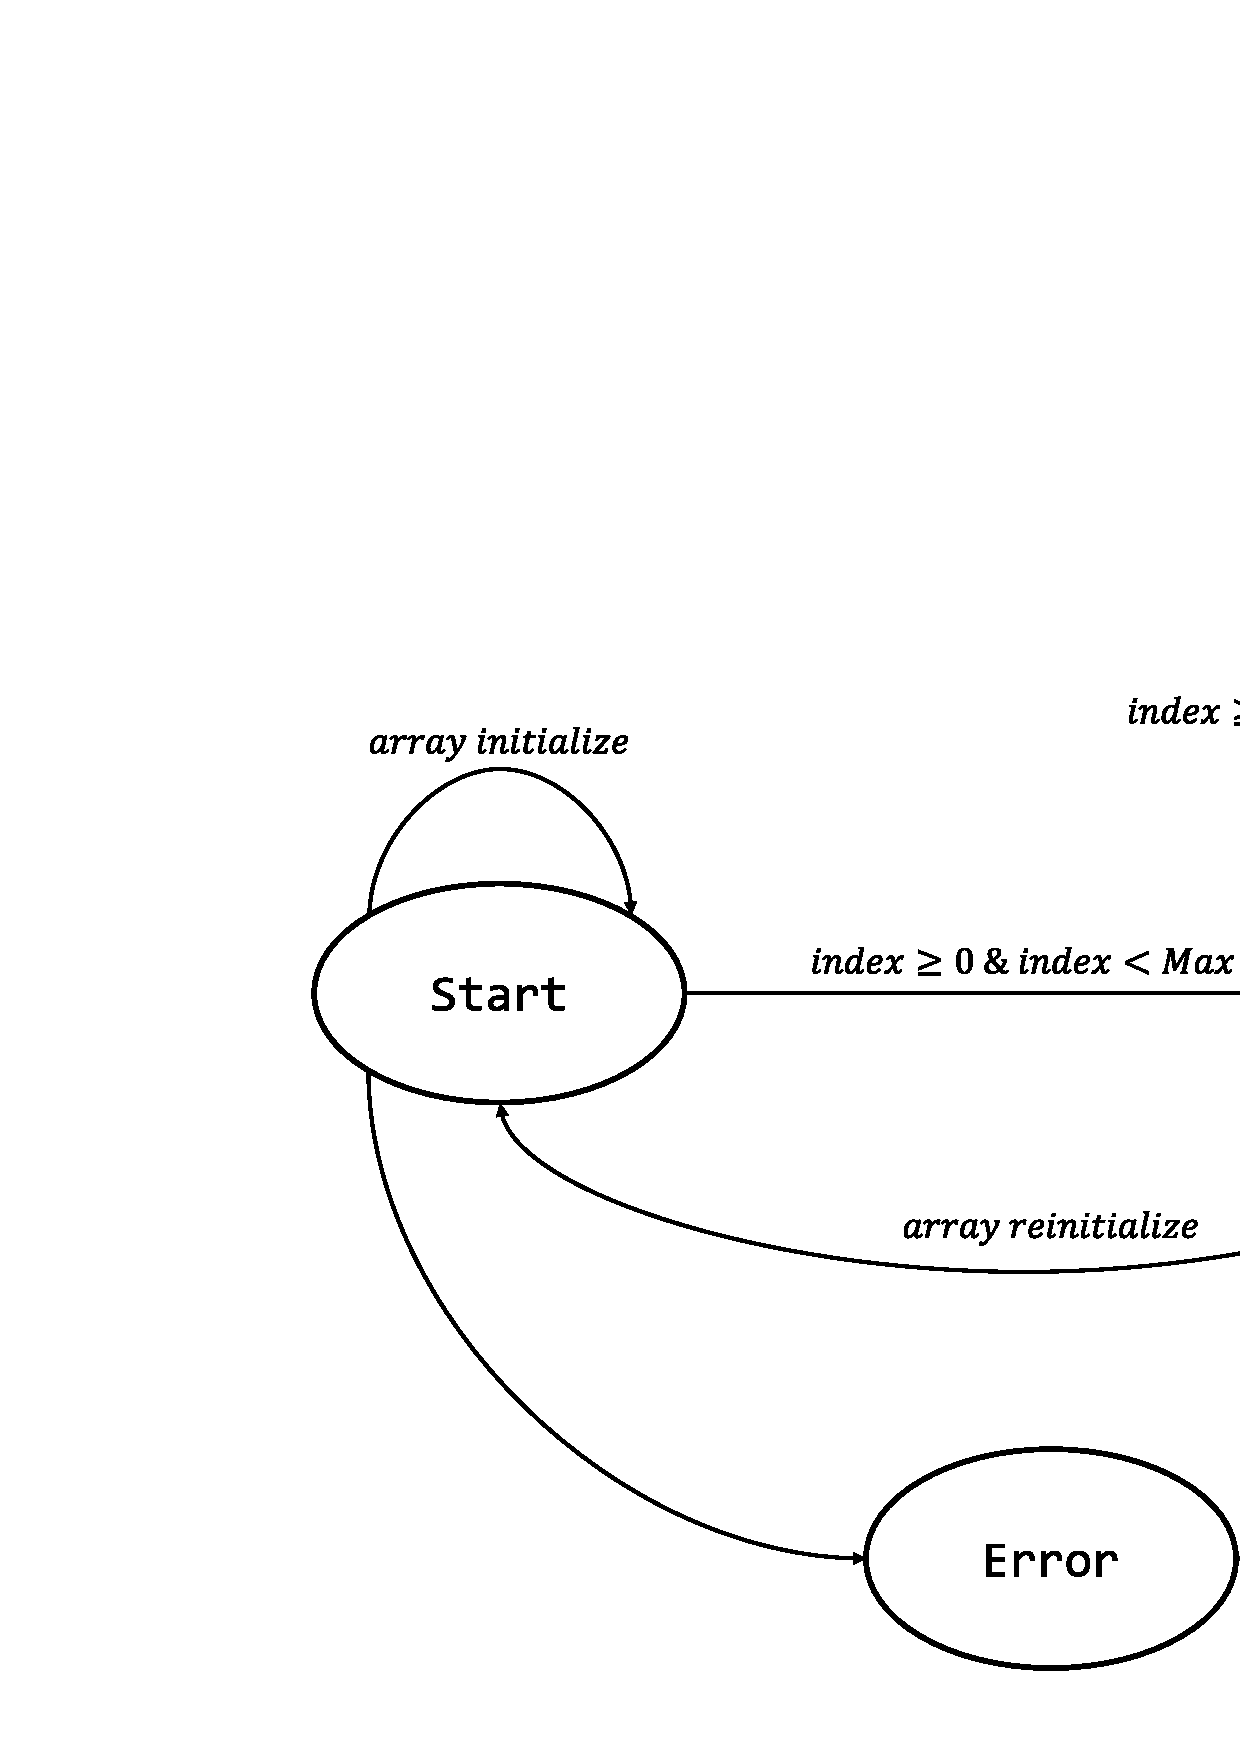
\includegraphics[scale = .25]{images/ArrayIndex.pdf}
\caption{array index out of bound formulated as FSM}
\label{fig:array}
\end{figure}


We can visualize all runtime exceptions as finite state machine (FSM). When a
program violates such sequence, it throws runtime exception. 
In Figure~\ref{fig:array}, array index out of bound (java.lang.
ArrayIndexOutOfBoundException) exception is described as a FSM. 
Here, a program will be in safe bound as long as the $array\_index \geq 0$ or
$array\_index \leq max\_array\_size - 1$

\subsection{Constraint Automata}
\label{subsec:constraintAutomata}

\emph{Constraint automata} is a formalism to describe the behavior and possible
data flow in coordination models. 
Mostly used for model checking. We have used it for the purpose of program
repairing technique. Here we define the finite state automata as follows :

$$(Q, \Sigma, \delta, q_0, F)$$
\begin{mybullet}
 \item $Q$: set of state where $|Q| = 2$, \emph{legal state}(init) and
\emph{illegal state} (error).
 \item $\Sigma$: symbols, invariants based on exception type.
 \item $\delta$: transition function. $init \rightarrow init$ is safe
transition and $init \rightarrow error$ is the invariant violation.
 \item $q_0$: starting state, here $q_0 = init$.
 \item $F$: end state, here it same as $q_0$.
\end{mybullet}

\begin{figure}[t]
\centering
\includegraphics[scale=.25]{images/automata.pdf}
\caption{Constraint automata general model}
\label{fig:automata}
\end{figure}

According to the Figure~\ref{fig:automata}, the repairing mechanism will only
trigger when we have a transition from 
init state to error state due to invariant violation.

\subsection{Patching Techniques}
\label{subsec:patchCA}

The patching technique is based on the exception type. 

%
\section{RepairingStrategy : Taint Analysis}
\label{sec:taintAnalysis}

We have used taint analysis to detect program paths between source-sink pair in
the program to determine which variables and objects go to tainted sink like
database, print stream, network stream etc. We have used InfoFlow framework and
modify it for our usage. The detaild design of the taint analysis module is
given in Chapter~\ref{chapter:SystemDesign}
Section~\ref{subsubsec:TaintingRule}. 

\subsection{Taint analysis : Definition}
\label{subsec:TaintAnalysisDef}

The term \textbf{taint} in the aspect of programming language is defined as
below:
\begin{definition}
Set of variables which are associated with program input is the set of tainted
variables.
\end{definition}
\begin{definition}
Variables which are associated or referenced from tainted variables are also
tainted.
\end{definition}
So, the set of variables are called as \textbf{tainted variable set} which may
trigger some undesirable events in the application.

\subsection{Taint analysis : Taint Propagation}
\label{subsec:TaintPropagation}

All tainted variables do not possess security threat. The tainted problem is
defined at three points. They are:

\begin{enumerate}
	\item Source descriptor $<m,n_s,p_s>$
	\item Derivation descriptor $<m,n_d,p_d>$
	\item Sink descriptor $<m,n_s,n_d,p_s,p_d>$
\end{enumerate}
Where $m$ is the method, $n$ is the number of parameter(s), $p$ is the access
path.$s$ and $d$ denotes to source and sink(destination) respectively.
\begin{figure}[t]
\centering
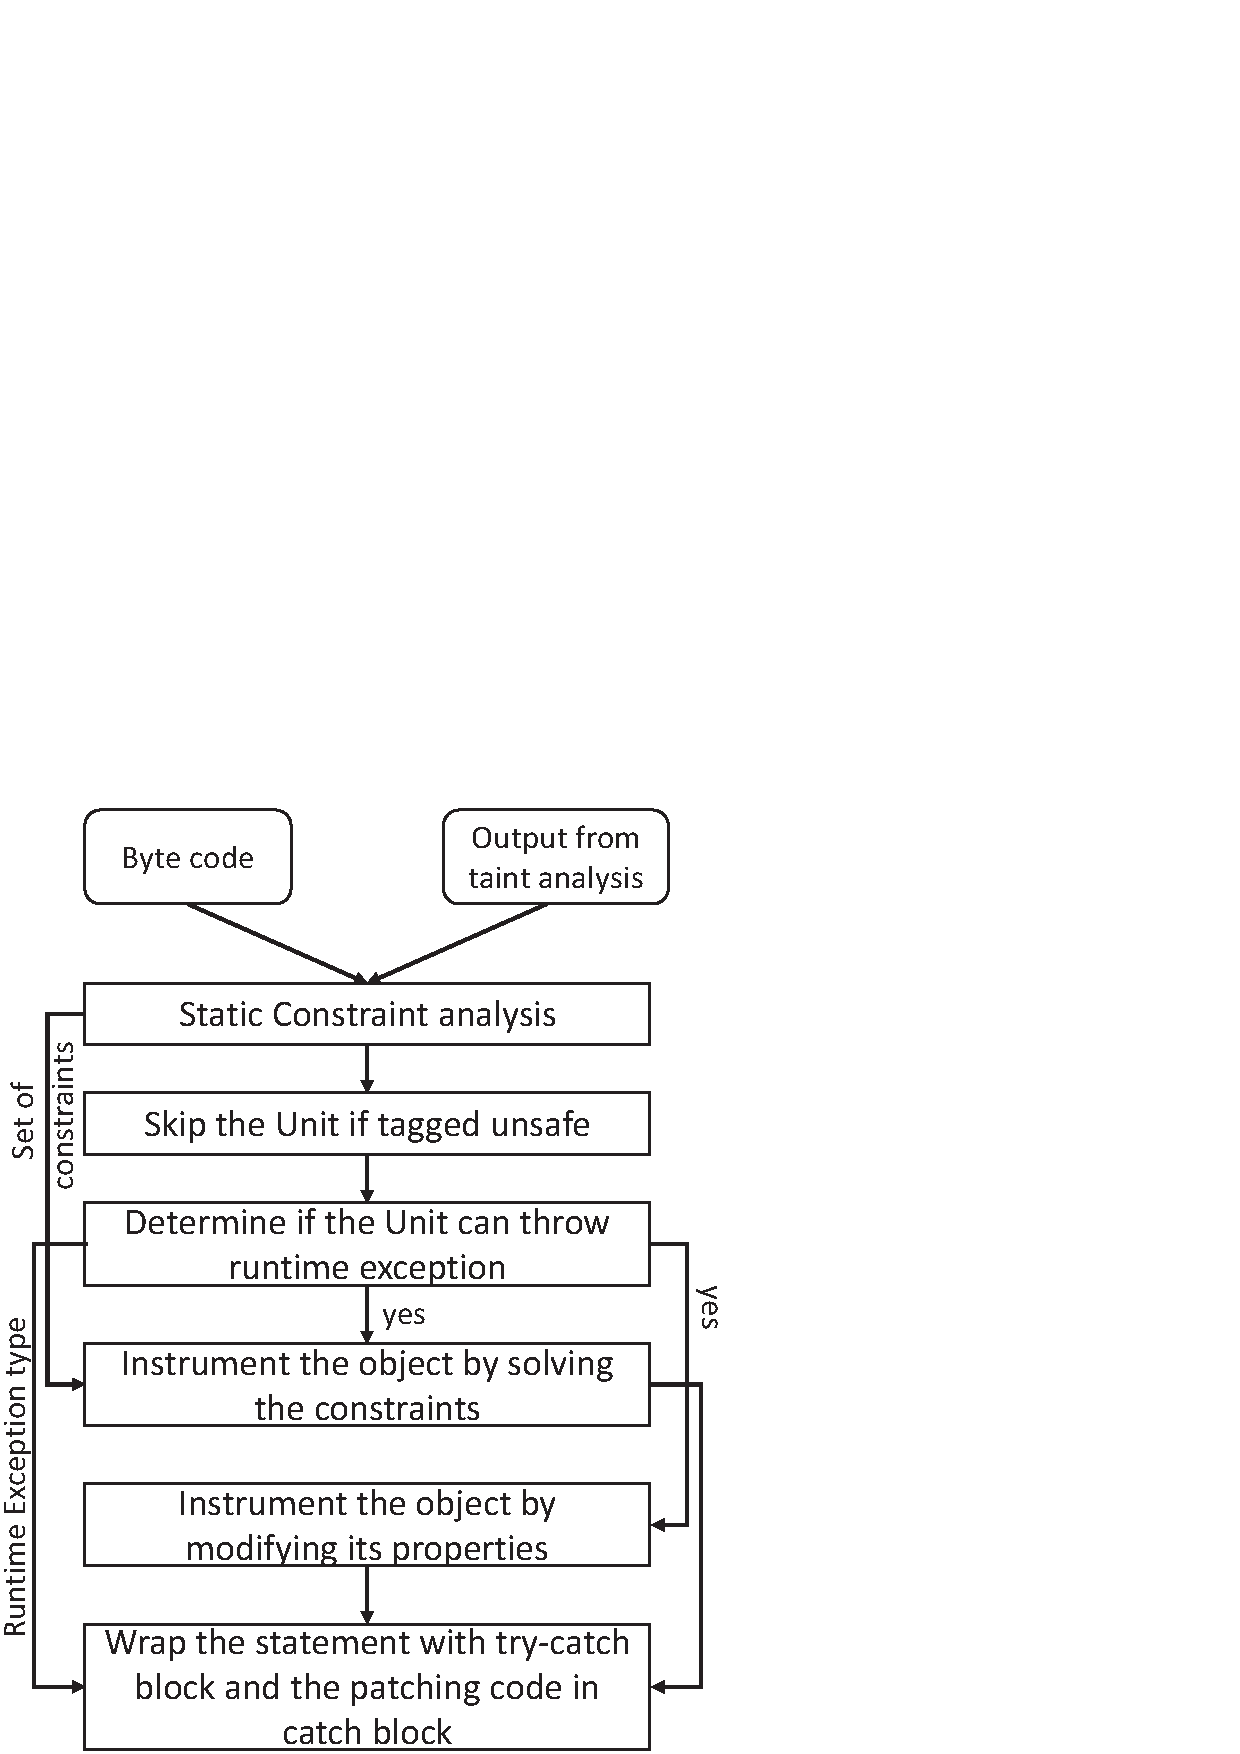
\includegraphics[width=5.5in]{images/PatchModule.png}
\caption{A simplified diagram indicating taint problem}
\label{fig:taint}
\end{figure}

\subsection{Taint Analysis : Relevance with Repairing Effort}
\label{subsec:TaintRepairing}

We have considered static taint analysis of the program (here we are analyzing
only java byte code) to eliminate any possibility of patching on the statements
which may go to some tainted sink like database, print stream or network stream.
Doing such we can ensure that the variables and objects we are patching will be
contained inside the system thus will not be leaked to outside. On such example
can be a client application on which we have done patching. Assume that we
patched a string object which was given as a input to the program. Due to some
formatting problem, the program throws a runtime exception. Ins uch scenario we
will regenerate the string object according to the constraint in the program to
make sure it stays very close to a clean input string. in any case the generated
string goes out from the system and used as a input to any external module it
may causes problem as the patched sting was solely designed for that particular
program. 

To avoid such cases we analyze the statement which in in the path of potential
tainted source and sink. In such cases we would not patch such statements.

%

\section{Repairing Strategy : Bounded Forward and Backward Analysis}
\label{sec:boundedAnalysis}

\subsection{Example Scenario}
\label{subsec:exampleScenario}

We have performed dataflow analysis by extending Soot main class. The objectives
of the dataflow analysis are the following:

\begin{itemize}
  \item For a target statement analyze used and defined variables.
  
  \item Extracts other statements which are both above and bellow the target
  statement in the control flow graph on which the used and defined variables
  are dependent on.
  
\end{itemize}

In the code snippet~\ref{snippet:dataflow}, we gave an example code based on java
\emph{String} API to demonstrate the analysis.


\lstset{language=Java, caption=Dataflow analysis,
label=snippet:dataflow}
\begin{lstlisting}
void bar()
{
  foo("fname:lname");
}

String foo(String s)
{
  int a = s.indexof(":");
  int b = s.indexOf("&");
  int c = s.indexOf("#");
  int d = 0;
  if(c>0)
  {
    d = 1;
  }
  return s.substring(a,b);
}

\end{lstlisting}

Let us assume that our target is \texttt{s.substring(a,b)} which in this case
may throw an array index out of bound exception. In this target statement,
\texttt{a} and \texttt{b} are used variable which are dependent on another
String API method i.e \texttt{indexOf()} which calculates index of starting of a
sub-string or single character in the main string. In case the sub-string or the
character does not exist in the main string, \texttt{indexOf()} method returns
$-1$ which causes throwing a runtime exception in the \texttt{substring()}
method call.
\newline
By using dataflow analysis we try to understand how these different variables
are correlated and based on that how we can effectively apply patching technique
so the patching code will have very less footprint in the instrumented bytecode.
In the Section~\ref{subsec:boundedForward}, we have given detailed explanations
of such analysis.


\subsection{Flow Functions}
\label{subsec:flowFunctions}

\begin{figure}[htb]
\centering
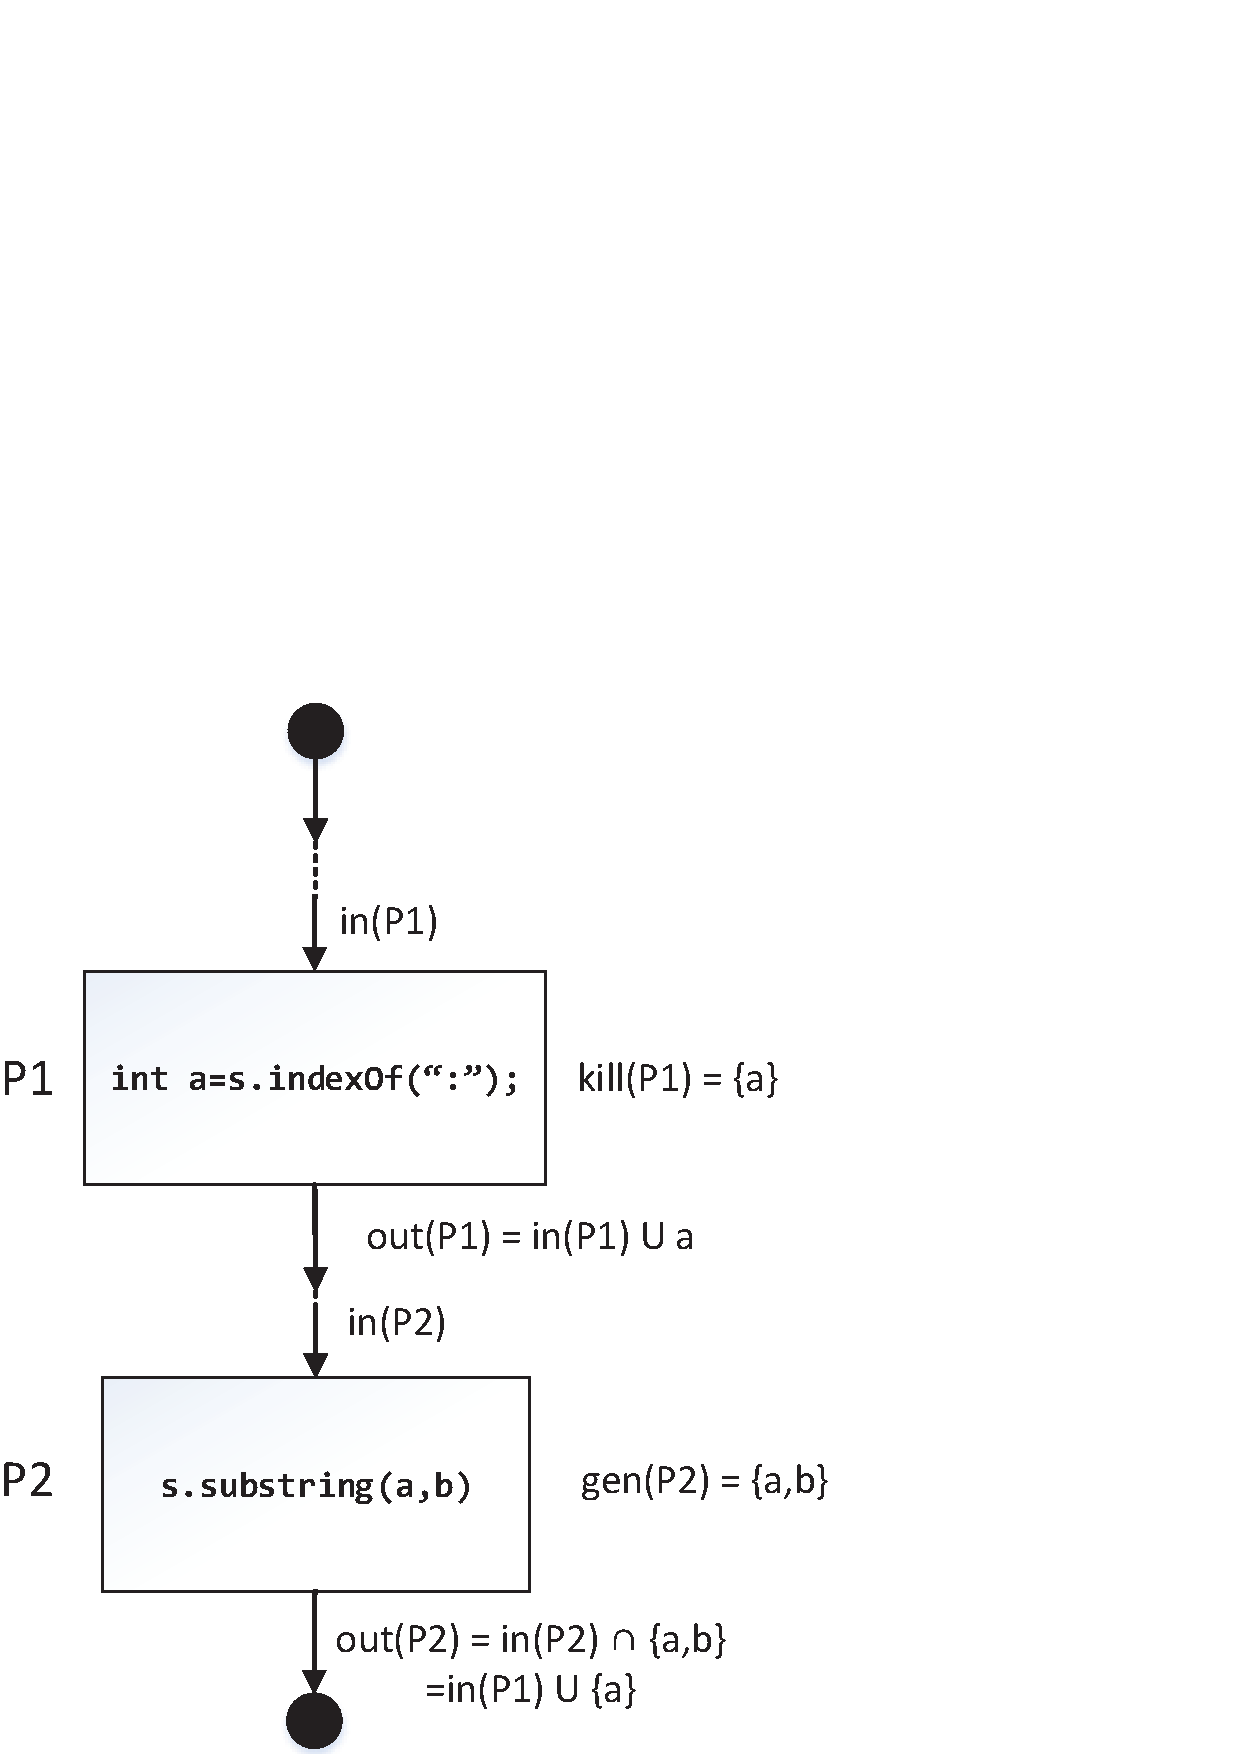
\includegraphics[width=3.2in]{images/dataflow.png}
\caption{Dataflow diagram with in, out set in forward analysis}
\label{fig:dataflow}
\end{figure}

\subsection{Bounded Forward Analysis}
\label{subsec:boundedForward}

Let us define $P_i$ as a program point/ node in the control flow graph. $in(P)$
and $out(P_i)$ respectively denotes in set and out set to and from the node $P$.
We define set $IG$ as the set of methods like \texttt{indexOf()},
\texttt{codePointAt()}, \texttt{CodePointBefore()} etc. which returns an integer
which can be used as input to other String methods. We also define set $IU$
which contains the methods which may use the integers produced by the methods in
$IG$ Then, 
$$out(P_i) = in(P_i) \cup Def(P_i)$$ where statement in P is a invoke statement
and method $m \in IG$ and
$$out(P_i) = in(P_i) \cap Used(P_i)$$ where statement in P is a invoke statement
and method $m \in IU$. Initial entry set = ${\phi}$.


We have defined $Def(P_i)$ set as the set of variables and objects which are
defined or redefined in the program point $P_i$. The set $Used(P_i)$ is also a
set of variables and objects which are used in the program point $P_i$.

\textbf{Example : } Consider the program statement \texttt{Pi : int a = b.fun(c
d)}.
Here the variable \texttt{a} is initialized, so $Def(P_i)$ = \texttt{\{a\}} and
as
\texttt{b, c, d} are used, $Used(P_i) =$ \texttt{\{b, c, d\}}

In the figure~\ref{fig:dataflow}, we gave an example of a sample CFG with in set
and out set.

\subsection{Constraint Satisfaction}
\label{subsec:constraintSatisfaction}

Dataflow analysis plays an important role in preparing the patching. One
patching mechanism we have come up with \texttt{String} objects is tht by
solving constraints which may come up in future will produce patch of better
quality. More over, it is very easy to extend the solution to other objects type
based on their API and characteristics of conditions. One such example is given
in the following code snippet~\ref{snippet:constraintCheck}


\lstset{language=Java, caption=Better patching mechanism with constraint
satisfaction, label = snippet:constraintCheck}
\begin{lstlisting}

void foo(String s, int i, int j)
{
	String str = s.substring(i,j);
	//some operation
	if(str.length() > 12){
	  //do something..
	}
	Integer in = 0;
	try{
	  StreamReader isr = new InputStreamReader(System.in);
	  String sin = new BufferedReader(isr).readLine();
	  in = Integer.parseInt(sin);
	}
	catch(IOException ex){}
	if(str.length() <= in){
	  //do something..
	}
	if(str.startsWith(SomeStringObject)){
	  //do something
	}
}

\end{lstlisting}

In the code snippet~\ref{snippet:constraintCheck}, the statement at line no $4$
is \texttt{s.substring(i,j)}, which can throw a
\texttt{IndexOutOfBoundsException}. This statement requires patching whic
involves generating a string for the object reference \texttt{str}. But in the
progrm, in line numbers \texttt{7, 16} and \texttt{20}, there are threee
conditional statements on \texttt{str} which involves constraint on the length
and the prefix of the string. There may be some set of constraint which can be
evaluated before hand, like the condition in in line numbers \texttt{7} which
involve a constant integer. But there can be cases like the conditional
statement in line numbers \texttt{16} which is also a lenght constraint like the
former, but in involves another variable which is taken frrom console, i.e. the
variable will be evaluated in run time. In such cases we can defer the
constraint evaluation process for that paricular condition. We can evaluate all
the conditions befor it, which can be safely evaluated. When we reach line
number \texttt{16}, then the variable \texttt{tt} would be available and can be
used to reevaluate the string \texttt{str}.

\subsubsection{Constraint Storage}
\label{subsubsec:constraintStorage}

For each of the string object, we store in the way illustrated in the
Figure~\ref{fig:constraint}.

\begin{figure*}[htb]
\centering
\includegraphics[scale=.5]{images/constraint.eps}
\caption{String constraints storage format}
\label{fig:constraint}
\end{figure*}

Wen to evaluate a new string object we need bounds like the minimuma and maximum
length, the prefixes and the candidate characters and their relative position.
We keep minimum information to safely evaluate the string.

\subsubsection{Constraint Evaluation Strategy}
\label{subsubsec:constraintStorage}

\begin{algorithm}
\DontPrintSemicolon
\KwData{String object $Str$ and constraint set $CS$.}
\KwResult{String object $Str$ such that $\forall i \in CS$, $Str$ satisfies $i$
}
\Begin
{
 $CS_{Str} \longleftarrow$ Get the constrint set for $Str$\;
 $MinLength \longleftarrow CS_{Str}[0]$\;
 $MaxLength \longleftarrow CS_{Str}[1]$\;
 $PrefixSet_{Str} \longleftarrow CS_{Str}[2 \rightarrow MaxLength + 1]$\;
 $ContainSet_{Str} \longleftarrow CS_{Str}[MaxLength +2  \rightarrow 2*MaxLength
 + 1]$\;
 
  \For{$C \in PrefixSet_{Str}$}
  {
   \If{$C$ is Empty}
   {
    continue\;
   }
   $PrefixLength \longleftarrow$ {\bf LENGTH OF} $C$\;
   
   \If{$PrefixLength$ is Maximum $\in PrefixSet_{Str}$}
   {
     Use $C$ to construct $Str$\;
   }
  }
 
  \For{$C \in ContainSet_{Str}$}
  {
   \If{$C$ is Empty {\bf OR} $C \in Str$}
   {
    continue\;
   }
   $Str \leftarrow Str$ {\bf APPEND} $C$\;
  }
  return $Str$\;
}
\caption{String object constraint evaluation}
 \label{algo:constraint}
\end{algorithm}

\subsubsection{Repairing Strategy using Constraint Evaluation}
\label{subsubsec:repairingStrategyConstraint}

The patching is evaluated in two ways, static and dynamic. We evaluated those
conditions which can be evaluated safely during compile time. Such constraints
have constants like \texttt{if(s.length<10)}. We looked for particular
constraints based on our storage specification 

%\section{Repairing Strategy : Constraint Automata}
\label{sec:strgCA}

\subsection{General Structure}
\label{subsec:generalCA}

\emph{Constraint automata} is a formalism to describe the behavior and possible data flow in coordination models. 
Mostly used for model checking. We have used it for the purpose of program repairing technique. Here we define the finite state automata as follows :

$$(Q, \Sigma, \delta, q_0, F)$$
\begin{itemize}
	\item $Q$: set of state where $|Q| = 2$, \emph{legal state}(init) and \emph{illegal state} (error).
	\item $\Sigma$: symbols, invariants based on exception type.
	\item $\delta$: transition function. $init \rightarrow init$ is safe transition and $init \rightarrow error$ is the invariant violation.
	\item $q_0$: starting state, here $q_0 = init$.
	\item $F$: end state, here it same as $q_0$.
\end{itemize}

\begin{figure}[!htb]
\centering
\includegraphics[width=3.2in]{images/automata.eps}
\caption{Constraint automata general model}
\label{fig:automata}
\end{figure}

According to the Figure~\ref{fig:automata}, the repairing mechanism will only trigger when we have a transition from 
init state to error state due to invariant violation.

\subsection{Patching Techniques}
\label{subsec:patchCA}

The patching technique is based on the exception type. 

\subsubsection{Array index out of bound exception}

Array index out of bound exception happen when one tries to access the array with a index which is more than the size of the array or 
less than zero i.e. with some negative value. We did the patching based on these two scenario. When the index is more than the array size, 
we patch it by assigning $array.length - 1$.

\lstset{language=Java, caption=array index out of bound patching, label=patchingexample2}

\begin{lstlisting}
void foo()
{
  int []arr = {1,2,3,4};
  int index = 10;
  int y = 0;
  try
  {
    //original code
    y = arr[index];
  }
  //patching instrumentation
  catch(IndexOutOfBoundException ex)
  {
    if(index > arr.length)
      y = arr[arr.length - 1];
    else
      y = a[0];
  }
}

\end{lstlisting}

\subsubsection{Negative Array Size Exception}

Negative array size exception occurs when one tries to create a array with a negative size. 
The patching is done based on data flow analysis. Suitable index size is determined by looking at the successive statement dependent on the array. 
To take a safe bound, we took maximum index size and set as the array size in the new array statement.


\lstset{language=Java, caption=arr index out of bound patching, label=patchingexample2}

\begin{lstlisting}
void foo()
{
  int []arr = {1,2,3,4};
  int index = 10;
  int y = 0;
  try
  {
    //original code
    y = arr[index];
  }
  //patching instrumentation
  catch(IndexOutOfBoundException ex)
  {
    if(index > arr.length)
      y = arr[arr.length - 1];
    else
      y = a[0];
  }
}

\end{lstlisting}

\subsubsection{Arithmetic Exception : Division-by-zero Exception}

Division by zero causes arithmetic exception. There are two different cases which were considered here. 
\begin{itemize}
	\item \textbf{Case I :} The denominator is going to the taint sink but the left hand side is not going to any taint sink. 
	Here we will not manipulate the denominator as we are not manipulating any variable which are going to any taint sink.
	\item \textbf{Case II :} The denominator and the left hand side, both are not going to any taint sink. So they are safe to patch.
\end{itemize}

\lstset{language=Java, caption=arithmetic exception : division-by-zero patching, label=patchingexample2}

\begin{lstlisting}
void foo()
{
  int a = 10;
  int b = 0;
	int y;
  try
  {
    //original code
    y = a/b;
  }
  //patching instrumentation
  catch(ArithmeticException ex)
  {
    //case I
    if(taintSink(b))
      y = 0;
    //case II
    else
    {
      b = 1;
      y = a/b;
    }
  }
}
\end{lstlisting}

\subsubsection{Null Pointer Exception}

Null pointer exception in Java is the most common runtime exception encountered. 
Thrown when an application attempts to use null in a case where an object is
required. There exists various scenarios where null pointer exception can
happen. These different scenario requires different patching techniques. Bellow
we enlist all cases and corresponding patching techniques.


\begin{itemize}
  \item \textbf{Case I} Calling the instance method of a null object. \newline
  \textbf{Patch :} This is patched by calling the constructor. In case there
  exists more than one constructor then we need to find most appropriate
  constructor. This is done by using data flow analysis in the successive
  statement to see which fields/methods been accessed and according to that
  most suitable constructor should be picked up, this will ensure safest way to
  deal with the later method calls/field accesses.
  
  \lstset{language=Java, caption=appropriate constructor, label=patchingexample2}

\begin{lstlisting}
class MyClass
{
 Integer field1;
 String field2;
 Double field3;

 public MyClass()
 {
  this.field1 = 1;
  this.field2 = null;
  this.field3 = null;
 } 
 public MyClass(Integer field1, String field2)
 {
  this.field1 = field1;
  this.field2 = field2;
  this.field3 = null;
 } 
 public MyClass(Integer field1, String field2, Double field3)
 {
  this.field1 = field1;
  this.field2 = field2;
  this.field3 = field3;
 }
 public Double getfield3()
 {
  return this.field3;
 }
}

class main
{
 Myclass mclass = null;
 Double a = null;
 try
 {
  //original code
  a = mclass.getfiled3() + 5.0;
 }
 //instrumentation
 catch(NullPointerException ex)
 {
  //choose appropriate constructor
  mlass = new MyClass(1, "a", 1.0); 
  a = mclass.getfiled3();
 }
}
\end{lstlisting}
  \item 
  
  \item \textbf{Case II} Possible Accessing or modifying the field of a null
  object.\newline
  \textbf{Patch :} The patch is same as the previous one.
  
  \item \textbf{Case III} Taking the length of null as if it were an
  array.\newline
  \textbf{Patch :}The patch for this situation is very much similar to the
  negative array size exception. Here we will do a data-flow analysis to see all
  the successive statements where the array object has been used (read or
  write). For safety we will take the maximum index from those statements and
  reinitialize the array object with the size.
    
  \lstset{language=Java, caption=array null pointer exception,
  label=patchingexample2}

\begin{lstlisting}
int[] bar(int a)
{
 int []arr = new int[a];
 int []b = (a > 10) ? arr:null;
 return b; 
}
void foo()
{
 int[] arr;
 int []arr = bar(5);
 try
 {
  //access or modify any field of arr
  //this will throw a null pointer exception
 }
 //instrumented code
 catch
 {
  int ARRAY_SIZE = 11;
  int []arr = new int[ARRAY_SIZE];
  //access or modify any field of arr
 }
}
\end{lstlisting}

  \item \textbf{Case IV} Accessing or modifying the slots of null as if it were
  an array.
 \textbf{Patch :} The patching mechanism is exactly same as before.
 
  \item \textbf{Case V} Throwing null as if it were a Throwable value.
\end{itemize}



%%%%%%%%%%%%%%%%%%%%%%%%%%%%%%%%%%%%%%%%%%%%%%%%%%%%%%%%%%%%%%%%%%%%%%%%%%%%%%%%%%%%%%%%%%%
%%%%%%%%%%%%%%%%%%%%%%%%%%%%%%%%%%%%%%%%%%%%%%%%%%%%%%%%%%%%%%%%%%%%%%%%%%%%%%%%%%%%%%%%%%%

\section{\tool}
\label{sec:tool}

\subsection{Goals}
\label{sec:tool:goals}

We identify the broad design goals for a technique to automatically repair
malformed strings or incorrect handling of strings as follows:

% i) identifies the statements which might be vulnerable to string-related errors,
% and are less critical to the functionality of the application such that
% suboptimal behavior might be acceptable,
% iii) generates patches by identifying constraints on the string data and if
% required, tweaks \code{String} API  parameters to regenerate legally correct
% string data,
% iv) optimizes the number of statements to be patched by retaining only the ones
% that need to be protected,  

\myparagraph{(i) High patch fidelity} We require that the patched program must
preserve the intended program behavior, \ie\ the patch must be precise and
should not induce any undesirable control flows in the repaired program.

\myparagraph{(ii) Non-invasive instrumentation} We require that the technique
must ensure no side-effects during normal program execution and activate patches
only when the program is guaranteed to crash.

\myparagraph{(iii) Low system overhead} We desire that the patched program must
incur no runtime overhead during normal program execution and only negligible
overhead in case of failures.

\subsection{Design}
\label{sec:tool:design}

\begin{figure}[t]
\centering
\includegraphics[scale=.38]{images/NewDesignDiagram.pdf}
\caption{\tool\ workflow.}
\label{fig:overallDesign}
\end{figure}

\myparagraph{\underline{Key Idea}} \tool\ leverages precise taint analysis and
call graph analysis to identify program instrumentation points, and builds upon
custom algorithms to generate targeted, high quality patches for repairing
programs with potential runtime exceptions, while still satisfying goals
mentioned in \xref{sec:tool:goals}.

Figure~\ref{fig:overallDesign} shows \tool's workflow, which involves three
main stages. First, \tool\ uses precise program analysis techniques to identify
points of interest, \ie\ string objects or API arguments that must be repaired
to prevent runtime exceptions. In the second stage, \tool\ leverages novel
custom algorithms to generate relevant patches. Specifically, \tool\ performs
intra-procedural static and dynamic analyses to identify and evaluate
constraints on the string objects under consideration. Third, \tool\ uses the
constraints evaluated in the earlier stage to programatically generate and embed
patches inside \texttt{catch} blocks to ensure that they do not get activated
during normal program execution.

\subsubsection{Precise Identification of Instrumentation Points}
\label{sec:tool:stage1}

In this stage, \tool\ leverages a combination of program analyses to accurately
determine the minimum set of points of interest where instrumentation is
required to repair. We list several techniques below that help \tool\ achieve
precision.

\myparagraph{(i) Taint analysis}: The main purpose of taint analysis is to
broadly identify which program statements can be patched (possibly even
suboptimally) without affecting the program control flow, \ie\ affect only
objects that are generated and stay within the application throughout their
lifetime. While this principle is not a binding constraint, it ensures that
\tool's repairing mechanism does not adversely affect critical program behavior.
We specify a generic set of sensitive sources and sensitive sinks for each input
program, to identify critical program paths where a repaired \code{String}
objects (and thus possibly suboptimal) must not flow. For example, \tool\ does
not repair program statements that lie along a control flow path that leads to
an I/O sink, like file system, console, network, GUI, etc.

\begin{table}[t]
\centering
\scriptsize
% \setlength{\tabcolsep}{3pt}
\begin{tabular}{l|l}
\multicolumn{1}{c|}{\textbf{Class}} & \multicolumn{1}{c}{\textbf{Source}}\\
\hline
\code{java.io.InputStream} & \code{read()}\\
\code{java.io.BufferedReader} & \code{readLine()}\\
\code{java.net.URL} & \code{openConnection()}\\
\code{java.util.Scanner} & \code{next()}\\
% \code{javax.servlet.http.HttpServletRequest} & \code{getParameter()}\\
\code{javax.servlet.ServletRequest} & \code{getParameter()}\\
\code{org.apache.http.HttpResponse} & \code{getEntity()}\\
\code{org.apache.http.util.EntityUtils} & \code{toString()}\\
\code{org.apache.http.util.EntityUtils} & \code{toByteArray()}\\
\code{org.apache.http.util.EntityUtils} & \code{getContentCharSet()}\\
\end{tabular}
\caption{Common sensitive sources in \java.}
\label{table:TaintSources}
\end{table}

\begin{table}[t]
\centering
\scriptsize
% \setlength{\tabcolsep}{3pt}
\begin{tabular}{l|l}
\multicolumn{1}{c|}{\textbf{Class}} & \multicolumn{1}{c}{\textbf{Sink}}\\
\hline
\code{java.io.FileOutputStream} & \code{write()}\\
\code{java.io.OutputStream} & \code{write()}\\
\code{java.io.PrintStream} & \code{printf()}\\
\code{java.net.Socket} & \code{connect()}\\
\code{java.io.Writer} & \code{write()}\\
\end{tabular}
\caption{Common sensitive sinks in \java.}
\label{table:TaintSinks}
\end{table}

The taint analysis module take as input the compiled byte code intended to be
repaired, and generates a control flow graph (CFG) identifying program
statements that lie along paths from sensitive sources to sensitive sinks.
Since, \tool\ targets strings in particular, it must support taint propagation
for all \java\ APIs that support string manipulation, including
\code{StringBuffer} and \code{StringBuilder}. All \code{String} objects (whether
generated or assigned) that lie along the tainted path from a sensitive source
to a sensitive sink are marked as \textit{unsafe} to patch. Subsequently, \tool\
does not repair such \code{String} objects. Figures~\ref{table:TaintSources} and
\ref{table:TaintSinks} list some common sensitive sources and sinks for several
classes in \java.

\myparagraph{(ii) Call graph analysis}:

\myparagraph{(iii) Optimizations}:


\ignore{
\paragraph{Identifying Program Statements.} We perform static taint analysis
to identify sensitive data which are leaving the system via database, network
stream, file stream or console. Providing patches to the
statements that manipulate this data would be undesirable, since
activation of the patches in case failures may allow altered sensitive data to
eventually
reach users. Hence, we only mark those program statements which do
not manipulate these data.

\paragraph{Noninvasive Patching.} In case a runtime exception that is thrown
by a statement as a result of a failure is already caught and handled in a
program,
we skip that statement from patching to avoid interfering with the results. Such
statements are identified by analyzing call-graphs and ensuring that no caller
method
in the call-chain handles the exception or its superclass. By embedding the
patches inside
\texttt{catch} blocks, we ensure that they do not get activated during normal
program execution.

\paragraph{Patch Generation.} We first perform an
intra-procedural static analysis
to identify constraints on the string objects under consideration. By
identifying
the type of exceptions that can be thrown in case of a failure, we
develop patches that
regenerate string objects by tweaking \java\ \code{String} API used in
the statements to regenerate legal string objects and by trying to solve the
constraints. In the latter case,
we evaluate the constraints statically if complete information is available at
the compilation-time. Otherwise, the analysis automatically generates
code that performs dynamic analysis to solve the constraints, and then
inserts this code in the generated patches.

\paragraph{Optimizing Instrumentation.} We perform reaching definitions
analysis to skip marked statements
if the string variables that are contained in the statements are already
patched, and the variables
are not redefined along any path that originates from the patched statement.
This analysis reduces
instrumentation points in a program.

\paragraph{Patch Precision.} The precision of a program patch is improved,
firstly, by targeting only strings
for patching which allows us to develop more specialized patches, secondly, by
patching programs very
close to the points of potential failures which avoids unnecessary patching of
other
unaffected variables and their potential
side effects, thirdly, by analyzing the types of exceptions that can be thrown
which
provides valuable insights into
origins of failures, and finally, by considering all the constraints
on the strings. This would result
in a program behavior closed to the intended one in case of a failure.

\paragraph{Reduced Overhead.} The side-effect of non-invasive patches is that
they do not interfere during
normal execution which results in no runtime overhead. Even when they get
activated in case of failures,
they still cause negligible overhead since we perform no analysis during runtime
except if required resolve the dynamic constraints.
As our study reveals~\xref{sec:evaluation} the constraints are typically few and
simple, making
the dynamic analysis light-weight.
}


\section{Implementation}
\label{sec:implementation}

We implemented a prototype of \tool\ as described in \xref{sec:design} for
repairing runtime exceptions originating from unhandled \java\ \code{String}
APIs. Our end-to-end toolchain is completely automated and was written in $x$
lines of \java. We leveraged the \soot~\cite{soot} framework for bytecode
analysis and instrumentation, and \infoflow~\cite{infoflow} for static taint
analysis.

% We have used our repairing strategy on the \java\ \code{String} API as it is one
% of the most frequent used APIs in commercially available \java\ applications and
% libraries. Another reason to choose \code{String} API was that we have found
% plenty of bugs related to \code{String} in some of the popular libraries and
% applications provided by Apache foundation, Eclipse, ASM etc.

We now briefly describe a few salient features of our implementation.

\subsection{Taint Analysis}

\infoflow\ performs its taint propagation over \code{Units}, which are \soot's
intermediate representation of the \java\ source code. We extended the
\infoflow\ framework to a) enable seamless coupling with \soot, and b) determine
whether it is safe to patch a given \soot\ \code{Unit}. Specifically, we added
a mapping that retrieves \code{Unit}s for statements to be patched given a
specified function signature. This is relevant since the same statement, say
\code{int x = 1;} has the exact same representation even if it appears in
multiple different functions. We also added a utility method to determine if a
\code{Unit} must be patched if it lies along the path between a source and sink
(recall Tables~\ref{tab:TaintSources} and ~\ref{tab:TaintSinks}) in the call
graph (as generated by \soot).

%  For the taint analysis phase we have used \soot\ \infoflow\ framework. This
%  framework requires configuration files to describe source and sink methods.
%  We
%  have identified couple of methods and some of them are tabulated in the
%  table~\ref{tab:TaintSources} and~\ref{tab:TaintSinks} respectively. We have
%  extended their InfoFlow class and added methods which store the statements in
%  a
%  \code{HashMap} object as \code{Unit}. The taint analysis phase takes two
% inputs: the jar file of the project which is to be analyzed and the
% \code{SootMethod}
%  signature of the entry point of that project.

\subsection{Constraint Analysis}
\label{subsec:constraint analysis}

Once the \infoflow\ taint analysis module identifies the \code{Units} to be
patched, \tool\ invokes its constraint analysis to determine the nature of the
patch. Specifically, patching involves a static component, which determines the
constraints by making a forward pass over the \code{Units} identified by the
taint analysis step, and a dynamic component, which is triggered if the
constraints could not be evaluated statically.

\subsubsection{Static Constraint Analysis}
\label{subsubsec:staticConstraint}

\tool\ performs static constraint analysis for all required \code{String}
objects to make the patched \code{String} as close to the ideal object. In this
phase, \tool\ analyzes all conditional statements on \code{String} literals to
statically determine a) prefix, b) suffix, and c) the length of the concerned
\code{String} literal. For example, \code{if(str.length() == 5} indicates that
for the program to enter the \code{True} branch of the conditional, \code{str}
must be of length $5$.

We collects all these information in a custom data type
and update it. For simplicity, we keep only the information such as minimum and
maximum length, set of characters which the string
may contains and set of possible prefix. With all these information, we generate 
the string object statically. The sting generation algorithm is described in
Algorithm~\ref{algo:constraint}. 

\subsubsection{Dynamic Constraint Analysis}
\label{subsubsec:dynamicConstraint}

We performed dynamic analysis in case the constraint can not be evaluated 
statically e.g. \code{if(str.contains(inputString()))}. In such cases just
before the conditional statement we instrument the bytecode with a static 
invocation which will populate the custom constraint data type and recalculate 
the string object with already existing constraints.

\subsection{String Repairing Phase}
\label{subsec:stringReepairing}

The string repairing phase is divided into two sub-phases.

\subsubsection{Detecting Potential Point of Failure}
\label{subsub:detectingFailure}

We have used specification from \java\ SE official documentation and list all
the methods which throws runtime exception. We do forward pass to see if there 
is any invocation of such methods and if we find any we then cross check it 
with the results we got from the taint analysis. We also see if there is already
some exception handling mechanism provided by the developer using the technique 
described in Section~\ref{subsec:callChainLookUp}. We detected such method calls
and wrap them in try-catch block. In the catch block we place the appropriate
exception type as provided by \java\ SE API documentation. 

\subsubsection{Catch Block Instrumentation}
\label{subsub:catchInstrumentation}

In this phase we instrument appropiate patching codes inside the catch block.
We used the static constraint evaluation of
Section~\ref{subsubsec:staticConstraint} to statically evaluate the string. In
cases there are more constraints which can't be solved statically, it would instrument
necessary method call so that the constraints would populate and get solved in runtime
~\ref{subsubsec:dynamicConstraint}. In case there is no constraint, we repair the
string in the method calls like \code{substrring}, \code{subSequence}, \code{charAt} etc.
which are dependent on the index arguments. In those cases we used
Algorithm~\ref{algo:stringPatchParametr} to repair them.


\begin{algorithm}
\scriptsize
\DontPrintSemicolon
\KwData{String object $Str$ and index set $IS$ which contains ${i}$ or
${i,j}$.}
\KwResult{Repaired index set containin ${Ri}$ or ${Ri,Rj}$ based on input $IS$}
\Begin
{
	$Length \longleftarrow$ length of $Str$\;
	\If{$Length == 0$} {
		$Ri, Rj \longleftarrow 0$\;
	} \Else {
		\If{$i \textgreater j$} {
			$Ri \longleftarrow j - 1$;
		}
		\If{$i \textgreater Lengrh$ \bf{OR} $j \textgreater Lengrh$} {
			$Ri \longleftarrow Length - 1$ or $Rj \longleftarrow Length - 1$ based on
			condition\; 
		}
		\If{$i \textless 0$ \bf{OR} $j \textless 0h$} {
			$Ri \longleftarrow 0$ or $Rj \longleftarrow 0$ based on
			condition\; 
		}		
	}	
}
\caption{String patching based on parameters passed}
\label{algo:stringPatchParametr}
\end{algorithm}
dfdf
ssfs

% 
% \subsection{Data Structures used in Various Phases}
% \label{subsec:dataStructure}
% 
% \begin{mylist}
% \item \textbf{Taint Analysis} : We kept \code{HashMap} object to store all the
% \soot\ \code{Unit} object corresponds to a \code{Boolean} value indicating
% the fact if the the \code{Unit} is safe to patch or not. In later phases we
% used this information. As we went through multiple phases of analysis and
% after each of the phases we did a \soot\ reset, we needed to make sure in the
% later phases object equality maintained for the \code{Unit} objects. To make 
% sure we kept the \code{PatchingChain} generated from the \code{Jimple} method
% \code{body} which is the representation of the control flow graph. For each of 
% the \code{Units}, me marked the position of it in the \code{patchingChain} to 
% make sure the comparison with the same \code{Unit} object in later phases also
% work properly. 
% 
% \item \textbf{Call Graph Analysis} : To detect already handled exception we
% see higher in the call chain if the call site of any one of the ancestors is
% wrapped in code{try-catch} block or not. To store and retrieve this information
% efficiently, we keep a \code{HashMap} where key is the method signature and 
% value is an \code{Object} array which contains a \code{Unit} and a \code{SootClass}.
% The \code{SootClass} object indicates the exception class by which the particular
% \code{Unit} was handled.
% 
% \item \textbf{Constraint Analysis} : We made a custom data type named \code{ConstraintDataType} 
% which contains the information of the constraint for a particular \code{String} object and also evaluate
% the sting when required. The data type has four fields of \code{Value} object which
% indicates the value corresponding to a \soot\ \code{Local} variable. These are minimum
% length, maximum length, an array of prefix and an array of contains (both \code{Character}
% or substring). To manage this data type, we used a \code{HashMap} which is indexed by the
% \code{String} object and the value is \code{ConstraintDataType}.
% 
% \end{mylist}


\subsection{Optimizations}
\label{subsec:optimizations}

\subsubsection{Call Chain Look-up for Already Handled Exception}
\label{subsubsec:callChainLookUp}

In some scenarios, the developer may put exception handling mechanism in case
there is any runtime exception. In such cases, we shouldn't do any repairing
as it may change the correct program behavior. There can be two cases.

\begin{mylist}

\item In the current method if the statement is wrapped in try-catch block. In
\soot\
the exception handling mechanism is handle by \code{Trap} class. Each
\code{Trap}
object has start, end and handler unit. From a particular \code{Unit}, we saw if
the unit belongs to any of the existing \code{Trap} and tag the \code{Unit} in
a \code{HashMap} object so that later at the repairing phase it can be exclude
from instrumentation.

\item If the exception is handled upper in the call chain, in the case we
generate
\code{CallGhaph} using the project's entry point as the entry point of that call
graph. For a method we did reverse Breadth First search (BFS) to see from which
methods it is invoked and also all of its ancestors in the call chain. From
there
we retrieve the information if any particular call sight was wrapped in
try-catch
block or not. In such case we tag the \code{Unit} in the \code{HashMap}
mentioned
before.

\end{mylist}

% \subsubsection{Minimize Patch Instrumentation}
% \label{subsubsec:minimizePatchInstrumentation}
% 
% To reduce number of instrumentation, we analyzed if all the statements which can
% throe runtime exception really requires shielding or not. After an
% instrumentation
% we observed if a particular string object is getting modified or not. In the
% case it
% is not modified and going through same string operation, it does not require any
% patching.
% 
% \subsubsection{Minimize Conflicts in Constraint Evaluation}
% \label{subsubsec:minimizeConflictsinConstraintEvaluation}
% 
% During the constraint evaluation both statically and dynamically, we
% instrumented
% methods calls which collect the information about the objects. To reduce
% conflicts at the time of evaluation
% we skipped some branches in which there are some thrown exception or error
% condition like
% \code{System.err.print()}. We only consider the conditional expressions in the
% branches having
% no exception or error pah.
% 
% \subsubsection{Minimize Constraint Instrumentation}
% \label{subsubsec:minimizeConstrintInstrumentation}
% 
% We instrument statements by which we can generate new string objects based on
% the
% constrains we observed in a forward pass of the program. In case a particular
% string object have not encountered any exception, we deferred the
% instrumentation
% until the first repairing instrumentation. There may be cases that the string
% object never went through such methods which can throw runtime exception, in
% such cases those instrumentation are not necessary.


\section{Evaluation}
\label{sec:results}


\subsection{Experimental Setup}
\label{sub:experimentalSetup}

We have looked to several bug repositories like Bugzilla, Apache issue tracker,
Eclipse project issue tracker etc and noticed number of bugs with major,
minor, critical and blocker priorities. We took choose several bugs from them
considering couple of facts
\begin{mylist}

\item \textbf{Popularity}: How much it is used among the developers and
industries,
\item \textbf{Severity} : We consider major, critical and blocker priority bugs
only considering the facts at the bug affects dependent applications and other
libraries severely.
\item \textbf{Age and state} : We consider latest bugs which were reported in
the last 5 years.
We also consider such bugs which still remains un-fixed.

We did all the experiments in a laptop pc equipped with a dual core Intel i5
2.3-2.9 GHz processor, 8 GB or RAM, Microsoft Windows 8.1 operating system, JDK
version 1.7-45 with 2 GB of allocated heap space. All the bug reproduction was done on
Eclipse Juno IDE. For static analysis and instrumentation we have used \soot\
version 2.5.0 and \soot\ \infoflow\ for static taint analysis. We have also used
java decompiler JD version 0.7.0.1. 

\end{mylist}


\subsection{Evaluation Matrices}
\label{sub:evaluationMartices}

We have conducted the evaluation based on the matrices which empirically
measures the precision and the performance of the developed tool. We measures
the precession in terms of the quality of the patch and some other criteria
listed bellow and the performance based on the time taken and the memory
footprint.

\begin{mylist}

\item \textbf{Patch similarity with the developers' patch} : This matrix is for
the qualitative analysis of our auto generated patches. By this measurement we
have not only ensure the effectiveness of the patch but also look at the
similarity of logic an patch construction with the developers' one.After the
patching we compared both the auto-generated patch code with the developer's
patching code we found in the bug repositories. In the case the bug is still
un-fixed we looked for the comments and discussion in the panel and collects
the information about the potential patch. At the first step, we visually
compared the patches to see how much they are similar and dissimilar with the
developers' patch. We than use the instrumented class files and place it to the
library archive replacing the buggy class files. We reproduced the similar test
cases of the bugs and used the automated patched version and later fixed version
of the same library to compare the results. In case the results are the primitive
or string type we have printed the output in the console and compare them. In
case the output is some complex object we compare the properties of them. Apart
from the test cases to reproduce the bug, we also ran couple of good test case
to make sure that the patch is not behaving any other way. Based on this
experiment we made a metric named \textbf{Patch Quality Index (PQI)} which
can contains three values, high, medium and low where we consider high PSI being
a good close quality patch.

\item \textbf{Auto-generated patch size and the develops' patch size} : Apart
from the qualitative analysis we have measured quantitative aspect of the
Auto-generated patches and compared their sizes with the developers' one.
Quantitative measurement comes to picture only when we are satisfied with the
qualitative measurement. We came up with a metric called \textbf{Patch Size
Index (PSI)}. In case our patch is qualitatively satisfactory and the size is
less than the developer one the we assign PSI as high. In case the size varies
in $\pm5\%$ we assign PSI as medium. If our patch is more than $5\%$ bigger than
the develops' one then PSI is assigned to low.

\item \textbf{Already handled exception} : We have analyzed the call graph to
see higher in the call chain or in the same method if a particular statement is
handled or not. In such cases we have abort our patching effort considering that
the exception is caught with exact exception type or its base type. We have also
done measurement to see if the patching actually disrupts the normal program
flow or not and we made a metric called \textbf{Program Flow Consistency Index
(PFCI)} which is calculated as
$$PFCI = \frac{Patch_{HE}}{Stmt_{HE}}$$

where $Patch_{HE}$ = Total number of patch placed in already handled exceptions,
and $Stmt_{HE}$ =  total number of statements in the program which are already
handled and $0 \le PFCI \le 1$. The lower value of $PFCI$ is desirable.


\item \textbf{Cascaded exception} : Cascaded exception can be a result of 
auto-generated patching in the case the patched objects are used as a input
to other methods and violates the specification there. This is the limitation
in our technique in the some complicated cases where it requires develops' 
attention. The limitation is due to the fact that the analysis for the repairing 
technique is a intra-procedural analysis and the constraint evaluation method is
very simple. For the constraint evaluation part, the solver is pluggable, we can
easily replace it with a third party solver. Cascaded exception can be noticed 
when the string object we are patching is generation some specific URI or driver
string which would be used to load or configure something. In such scenario, the
patch may produce some malformed string. In case there is a cascaded exception 
in string object, our analysis will take care of it, other wise it would abort. 

\item \textbf{Time} : For each of the analysis phase, we record the time taken.

\item \textbf{Memory Consumption} : Similarly we monitored memory consumption
for all of the phases in the analysis.

\end{mylist}

\begin{sidewaystable}
%\small
\begin{tabular}{@{\makebox[3em][r]{\rownumber\space}}|l|c|c|c|c|c|c|c|c|c|c|c|c|c|c}
\multicolumn{1}{c|}{\textbf{API}} &
\multicolumn{1}{c|}{\textbf{BugID}} &
\multicolumn{1}{c|}{\textbf{Priority}} &
\multicolumn{1}{c|}{\textbf{$PQI$}} &
\multicolumn{1}{c|}{\textbf{$PSI$}} &
\multicolumn{1}{c|}{\textbf{$PFCI$}} &
\multicolumn{1}{c|}{\textbf{$LOC$}} & 
\multicolumn{1}{c|}{\textbf{$IC_O$}} & %instrumentation with optimization
\multicolumn{1}{c|}{\textbf{$IC_{UO}$}} & %instrumentation without optimization
\multicolumn{1}{c|}{\textbf{$\mathcal{N}_{CG}$}} &
\multicolumn{1}{c|}{\textbf{$PF_{TA}$}} & 
\multicolumn{1}{c|}{\textbf{$PF_{CG}$}} &
\multicolumn{1}{c|}{\textbf{$PF_{CA}$}} &
\multicolumn{1}{c|}{\textbf{$PF_{IN}$}} &
\multicolumn{1}{c}{\textbf{$\mathcal{N}_{CE}$}}\\ % cascaded exception


\hline
\code{Aries} 	 	  		& \cite{ARIES1204} & Major 	& High & High & $0$ &$129$ &$42$
& $42$ & $3496$& & &&&\\
\code{Commons CLI1.x}  		& \cite{CLI46} & Major 	&  &  & & & & & & & &&&\\
\code{Commons CLI2.x}  		& \cite{CLI193} & Major 	&  &  & & & & & & &&& &\\
\code{Commons Compress}		& \cite{COMPRESS26} & Blocker &  &  & & & & & & &&& &\\
\code{Commons IO}   		& \cite{IO179}  & Major 	&  &  & & & & & & & &&&\\
\code{Commons Lang} 	  	& \cite{LANG457}& Major 	&  &  & & & & & & & &&&\\
\code{Commons Math} 	  	& \cite{MATH198} & Major 	&  &  & & & & & & & &&&\\
\code{Commons Net} 	  		& \cite{NET442} & Major   &  &  & & & & & & & &&&\\
\code{Commons VFS} 	  		& \cite{VFS338} & Major 	&  &  & & & & & & & &&&\\
\code{Eclipse AspectJ} 		& \cite{EclipseBug333066} & Major 	&  &  & & & & &
&&&&&\\
\code{Hive} 			  	&\cite{}& Major 	&  		  &  & & & & & & & &&&\\
\code{HttpClient} 	  		&\cite{HTTPCLIENT150}& Major 	&  &  & & & & & & & &&&\\
\code{jUDDI} 	  			&\cite{JUDDI292}& Major 	&  &  & & & & & & & &&&\\
\code{Log4j} 		  		&\cite{ApacheLog4jBug}& Major 	&  &  & & & & & & &&& &\\
\code{Pivot} 		  		&\cite{PIVOT533}& Major   &  &  & & & & & & &&& &\\
\code{Qpid} 			  	&\cite{}& Blocker &  &  & & & & & & & &&&\\
\code{Servicemix-soap} 		&\cite{SMXCOMP156}& Major   &  &  & & & &  & &&&& &\\
\code{SOAP} 			 	&\cite{SOAP130}& Major 	&  &  & & & & & & &&& &\\
\code{Struts2} 		  		&\cite{WW650}& Major 	&  &  & & & & & & &&& &\\
\code{Tapestry 5} 		  	&\cite{TAP51770}& Major 	&  &  & & & & &&& & & &\\
\code{Wicket} 		  		&\cite{WICKET4387}& Major 	&  &  & & & & &&& & & &\\
\code{XalanJ2} 		  		&\cite{XALANJ836}& Major 	&  &  & & &  & && &&& &\\

\end{tabular}

\caption{Experimental results}
\label{tab:results}
\end{sidewaystable}

\section{Related Work}
\label{sec:relatedWork}

There has been considerable amount of research done in the area of automated
program repairing. The approaches that have been proposed by the researchers
broadly fall into two categories namely, static and dynamic.

The static approaches work based on the counter-example or the violated
invariants that are reported from the field. These approaches then repair the
program by automatically developing a patch and then ensure its correctness
using computationally intensive techniques such as model-checking
\cite{biere2014, wei-issta-2010}.
These techniques are effective in producing accurate patches. However, shutting
down the system to produce and apply patches is not always feasible or
desirable. To overcome these problems, several promising dynamic approaches have
been proposed. These approaches typically develop either suboptimal patches or
isolate the data structure that is damaged which allows at least part of the
system to be functional \cite{conf/issre/DemskyR03, conf/icse/DemskyR05,
conf/issta/DemskyEGMPR06}. The advantage of these approaches is that they are
light-weight and can fix the system on-the-fly. Long et al.
\cite{conf/pldi/LongSR14} have developed an approach that deals with two most
commonly observed software errors, and then suppressing the errors with the help
of a runtime that operates by first invoking a  signal handlers, and then by
running a dynamic symbolic execution to ensure no side-effects.
This approach is light-weight and like our approach fixes the errors on-the-fly
potentially allowing some sub-optimal behaviour for a finite time until the
systems self-stabilizes.
In contrast our approach targets only string objects for repairing allowing it
generate highly precise program patches which generate very few or none
cascading exceptional events and produces a program behavior which is very close
to the expected behavior under the event of crashing.
In addition, our approach is hybrid with a heavy static component which enables
all the analysis including the side-effect analysis based on a taint analysis to
perform dynamically. It incurs negligible overhead even in the event of
crashing.

%%added new
In the litarature there exists proir art where the authors used string
transformation and solving technique for repairing purpose. In the paper
\cite{Singh:2012}, the authors deals with semantic transformation of the string
like manipulating strings that need to be interpreted as more than a sequence of
characters, e.g., as a column entry from some relational table, or as some
standard data-type like date, time, currency, etc. In \cite{Gulwani:2011}, the
author designed a learning algorithm for learning a string expression that is
consistent with input output examples. The input output example is generated
from a mapping which maps a set of string to a string defining a operation like
concatenation. There are works on genetic programming technique like
\cite{LeGoues:2012Ex, LeGoues:2012, DBLP:journals/cacm/WeimerFGN10} where the
 technique generated program patch by using already existing test cases to deal
with bugs like infinite loop, null string, segmentation fault, buffer overflow
etc.

\ignore {
% % added from the mail : from PLDI author response

Automated repair of HTML generation errors in PHP applications using string
constraint solving

In this paper the authors proposed a technique to repair the auto generated
malformed HTML codes from the PHP scrips. Often the HTML codes do not have
proper tags which are silently corrected by the browser but the result is
different across browsers. The authors employed an efficient SAT solver named
Kodkod using cost optimization to find the best repair.
%%%%%%%%%%%%%%%%%%%%%%
Deep Typechecking and Refactoring

Here the authors focused on the java database API and related query string. They
proposed the solution of type errors which is caused due to the type mismatch in
the database and the type assigned in the program. The authors also proposed a
solution for refactoring where changing a class name associated with some
queries will reflect all the strings system wide.
%%%%%%%%%%%%%%%%%%%%%%%%
GenProg: A Generic Method for Automatic Software Repair

The author used genetic programming technique which is a stochastic search
method inspired by biological evolution. The technique generated program patch
by using already existing test cases to deal with bugs like infinite loop, null
string, segmentation fault, buffer overflow etc.
%%%%%%%%%%%%%%%%%%%%%%%%%
Automatic Program Repair with Evolutionary Computation

Same paper as the above (Journal version) written by same authors.
%%%%%%%%%%%%%%%%%%%%%%%%%%%%%
A Systematic Study of Automated Program Repair: Fixing 55 out of 105 Bugs for $8
Each

Extended work of the above. The paper deals with the real life feasibility if
GenProg like what fraction of the bugs it can repair and the cost associated
with it.
%%%%%%%%%%%%%%%%%%%%%%%%%%%
Automating String Processing in Spreadsheets Using Input-Output Examples

The author considered Microsoft Excel programs as the use case scenario and
identified string processing as the major class of programming problem which
includes names/phone-numbers/dates from one format to another, data cleansing,
extracting data from several text files or web pages into a single document,
etc. The author designed a learning algorithm for learning a string expression
that is consistent with input output examples. The input output example is
generated from a mapping which maps a set of string to a string defining a
operation like concatenation.
%%%%%%%%%%%%%%%%%%%%%%%%%%%%
Learning Semantic String Transformations from Examples

The authors deals with semantic transformation of the string like manipulating
strings that need to be interpreted as more than a sequence of characters, e.g.,
as a column entry from some relational table, or as some standard data-type like
date, time, currency, etc.


% %%%%%%%%%%%%%%%%%%%%%%%%%%%%%%%%%%%%%%%%%%%%%%%%%%%%%%%%%%%%%%%%%%%%%%%%%%%
Several approaches have been proposed in the past to ensure that programs can
recover from failures. Some of the approaches are based on static repairing
where the patches are synthesized automatically based on the counter examples
found in the field \cite{wei-issta-2010}.
However, it is not always desirable to shut down the system for the post-mortem
analysis and then relaunch it after fixing the defect. In order to overcome this
weakness, dynamic approaches have been proposed to deal with problems that are
related to memory, data, and incorrect programming constructs such as infinite
loops \cite{Carbin:2011, KlingMCR12, conf/sosp/PerkinsKLABCPSSSWZER09}. Some of
the approaches work either by identifying and isolating damaged data or memory
portions \cite{conf/issre/DemskyR03, conf/icse/DemskyR05,
conf/issta/DemskyEGMPR06}, or by delaying the execution until the program
self-stabilizes \cite{Eom:2012}, or by finding the alternative execution paths
\cite{PezzeRWZ11}, or by disabling suppressing signals and hoping that the
program can recover automatically from the errors \cite{conf/pldi/LongSR14}.
Static approaches strive for correctness whereas dynamic approaches are
typically optimistic and work on the assumption that some suboptimal behavior
under certain conditions is acceptable.

\myparagraph{Data Structure Repairing}
% \label{subsec:RecWorksDataStructure}
Demsky and Rinard have proposed approaches that repair data structures ~\cite{
Demsky03automaticdata, conf/issre/DemskyR03,conf/oopsla/DemskyR03,
conf/issta/DemskyEGMPR06} the authors mostly concentrated on specific
data-structures like \emph{FAT-32}, \emph{ext2}, \emph{CTAS} (a set of
air-traffic control tools developed at the NASA Ames research center) and
repairing them. The authors represented a specification language by which they
able to see consistency property these data-structure.
Given the specification, they able to detect the inconsistency of these
data-structures and repair them.
The repairing strategy involves detecting the consistency constraints for the
particular data structure, for the violation, they replace the error condition
with correct proposition. In the paper~\cite{conf/icse/DemskyR05}, the authors
Demsky et al. proposed repair strategy by goal-directed reasoning. This involves
translating the data-structure to a abstract model by a set of model definition
rules. The actual repair involves model reconstruction and statically mapped it
to a data structure update. In the paper~\cite{conf/oopsla/2007} authors
Elkarablieh et al. proposed the idea to statically analyze the data structure to
access the information like recurrent fields and local fields. They used their
technique to some well known data structures like singly linked list, sorted
list, doubly liked list, N-ary tree, AVL tree, binary search tree, disjoint set,
red-black tree, Fibonacci heap etc.

\myparagraph{Works on Software Patching}
% \label{subsec:RecWorksSoftPatch}
In their paper~\cite{conf/sosp/PerkinsKLABCPSSSWZER09}, authors Perkins et al.
presented their \emph{Clear view} system which works on windows x86 binaries
without requiring any source code. They used invariants analysis for which they
used Daikon~\cite{DBLP:journals/scp/ErnstPGMPTX07}. They mostly patched security
vulnerabilities by some candidate repair patches.

Fan Long et al. in their paper~\cite{conf/pldi/LongSR14} presented their new
system \emph{RCV} which recovers applications from divide-by-zero and
null-deference error. Their tool replaces \emph{SIGFPE} and \emph{SIGSEGV}
signal handler with its own handler. The approach simply works by assigning zero
at the time of divide-by-zero error, read zero and ignores write at the time of
null-deference error. Their implementation was on $x86$ and $x86-64$ binaries
and they also implemented a dynamic taint analysis to see the effect of their
patching until the program stabilizes which they called as \emph{error
shepherding}.

\myparagraph{Genetic Programming, Evolutionary Computation}
% \label{subsec:RecWorksGeneric}
Reserch works on program repair based on genetic programming and evolutionary
computation can be found in the paper of Forrest et al.s~\cite{conf/gecco/2009g}
and Weimer et al.~\cite{DBLP:journals/cacm/WeimerFGN10} respectively. In the
papers, the authors used genetic programming to generate and evaluate test
cases. They used their technique on the well known Microsoft Zune media player
bug causing the application to freeze up.
}




\section{Conclusion and Future Works}
\label{sec:conc}


%%\acks

\raggedright
\small
\bibliographystyle{abbrvnat}
\bibliography{paper}

\end{document}
